\documentclass[authoryear,5p]{elsarticle}

\renewcommand{\today}{}  % Get rid of date on footer
\journal{Ann. Nucl. Energy}

\usepackage[bitstream-charter]{mathdesign} % Use BT Charter font
\usepackage[T1]{fontenc}                   % Use T1 encoding instead of OT1
\usepackage[utf8]{inputenc}                % Use UTF8 input encoding
\usepackage{microtype}                     % Improve typography
\usepackage{amsmath, mathtools}             % AMS Math extensions
\usepackage{booktabs}                      % Improved table spacing
\usepackage{booktabs}
\usepackage{siunitx}
\usepackage{breqn}
\usepackage{nicefrac}
\usepackage{multirow}

\usepackage[breaklinks=true]{hyperref}

\usepackage{subcaption}
\usepackage{dblfloatfix}
\usepackage{color}

\usepackage{todonotes}

\usepackage[labelfont=bf]{caption}
\captionsetup[figure]{labelsep=period, name=Figure}
\captionsetup[table]{labelsep=period, name=Table}
\def \figureautorefname {Figure}
\def \algorithmautorefname {Algorithm}

\usepackage[scaled]{beramono}

\usepackage{etoolbox}
\usepackage{listings}
\usepackage{color}

% Algorithm constructs
\usepackage{algorithm} % Provides algorithm environment
\usepackage{algorithmicx}       % Provides algorithmic block
\usepackage{algpseudocode}      % Option of algorithmicx package
\renewcommand{\thealgorithm}{\thechapter-\arabic{algorithm}}
\newcommand\Algphase[1]{%
\vspace*{-.7\baselineskip}\Statex\hspace*{\dimexpr-\algorithmicindent-2pt\relax}\rule{\columnwidth}{0.4pt}%
\Statex\hspace*{-\algorithmicindent}{#1}%
\vspace*{-.7\baselineskip}\Statex\hspace*{\dimexpr-\algorithmicindent-2pt\relax}\rule{\columnwidth}{0.4pt}%
}
\newcommand{\algrule}[1][.4pt]{\par\vskip.5\baselineskip\hrule height #1\par\vskip.5\baselineskip}

\newcommand{\code}[2]{
  \subsection*{#1}
  \lstinputlisting{#2}
}

\def\sectionautorefname{Sec.}
\def\subsectionautorefname{Sec.}
\def\subsubsectionautorefname{Sec.}
\def\equationautorefname{Eq.}
\def\figureautorefname{Fig.}
\def\algorithmautorefname{Alg.}

% Patch to make equation autoref counter work
\makeatletter
\patchcmd\eq@setnumber{\stepcounter}{\refstepcounter}{}{%
  \errmessage{Patching \noexpand\eq@setnumber failed}%
}
\makeatother

\hypersetup{colorlinks=true,
  pdftitle={The Impact of Spatial Self-Shielding on Pin-wise Reaction Rates},
  pdfauthor={William Boyd, Benoit Forget and Kord Smith.}}

\begin{document}

\begin{frontmatter}

\title{The Impact of Spatial Self-Shielding on Pin-wise Reaction Rates}

\author{William Boyd\corref{cor1}}
\ead{wboyd@mit.edu}

\author{Benoit Forget\corref{}}
\ead{bforget@mit.edu}

\author{Kord Smith\corref{}}
\ead{kord@mit.edu}

\address{Massachusetts Institute of Technology, Department of Nuclear Science and Engineering, 77 Massachusetts Avenue, Building 24, Cambridge, MA 02139, United States\vspace{-8ex}}


%%%%%%%%%%%%%%%%%%%%%%%%%%%%%%%%%%%%%%%%%%%%%%%%%%%%%%%%%%%%%%%%%%%%%%%%%%%%%%%
\begin{abstract}
%%%%%%%%%%%%%%%%%%%%%%%%%%%%%%%%%%%%%%%%%%%%%%%%%%%%%%%%%%%%%%%%%%%%%%%%%%%%%%%

\end{abstract}

\begin{keyword}
Multi-group cross-sections, spatial homogenization, spatia self-shielding
\end{keyword}

\end{frontmatter}

%%%%%%%%%%%%%%%%%%%%%%%%%%%%%%%%%%%%%%%%%%%%%%%%%%%%%%%%%%%%%%%%%%%%%%%%%%%%%%%
\section{Introduction}
\label{sec:intro}
%%%%%%%%%%%%%%%%%%%%%%%%%%%%%%%%%%%%%%%%%%%%%%%%%%%%%%%%%%%%%%%%%%%%%%%%%%%%%%%

The nuclear reactor physics community has long strived for deterministic neutron transport-based tools for whole-core reactor analysis. A key challenge for whole-core multi-group transport methods is accurate reactor agnostic multi-group cross section (MGXS) generation. The MGXS generation process applies a series of approximations to produce spatially homogenized and energy condensed MGXS in each spatial zone and energy group. ... However, the practical impact of ... is less understood. This paper investigates the ... and quantifies its significance for heterogeneous PWR problems.

This work employs Monte Carlo (MC) neutron transport simulations to generate MGXS. Monte Carlo methods have increasingly been used to generate few group constants for coarse mesh diffusion, most notably by the Serpent MC code \citep{serpent2013manual}, and to a much lesser extent, for high-fidelity neutron transport methods~\citep{redmond1997multigroup, nelson2014improved, cai2014condensation, boyd2016thesis}. The advantage of a MC-based approach is that all of the relevant physics are directly embedded into MGXS by weighting the continuous energy cross sections with a statistical proxy to the ``true'' neutron flux. 

This paper seeks to identify the bias between continuous energy and multi-group transport methods for MGXS libraries which account for spatial self-shielding effects\footnote{The effects of neighboring pins, burnable poisons, reflectors and the core baffle are each of interest in the context of spatial self-shielding.} to varying degrees. In particular, this paper quantifies the difference in the approximation error between simulations in which the same MGXS are used in each unique fuel pin (\textit{e.g.}, each fuel enrichment) and those in which unique MGXS are used in each and every pin. The former case does little if anything to model spatial self-shielding effects, whereas the latter case ``fully'' resolves these effects, albeit at the expense of very large MGXS libraries.

% This difference in approximation error motivates the development of a novel methodology in the following chapters which uses statistical clustering to capture spatial self-shielding effects in MGXS.

The content in this paper is organized as follows. Two different schemes for spatial homogenization of pin-wise MGXS are introduced in~\autoref{sec:methodology}. The need for a new, more flexible and specialized approach to spatial homogenization which appropriately captures spatial self-shielding effects with minimal computational expense is discussed in~\autoref{sec:conclusions}.
%%%%%%%%%%%%%%%%%%%%%%%%%%%%%%%%%%%%%%%%%%%%%%%%%%%%%%%%%%%%%%%%%%%%%%%%%%%%%%%
\section{Methodology}
\label{sec:methodology}
%%%%%%%%%%%%%%%%%%%%%%%%%%%%%%%%%%%%%%%%%%%%%%%%%%%%%%%%%%%%%%%%%%%%%%%%%%%%%%%

%%%%%%%%%%%%%%%%%%%%%%%%%%%%%%%%%%%%%%%%%%%%%%%%%%%%%%%%%%%%%%%%%%%%%%%%%%%%%%%
\subsection{Continuous Energy Calculations with OpenMC}
\label{subsec:openmc}

-OpenMC~\cite{romano2013openmc}
-Python API~\cite{boyd2016bigdata}
-NNDC data~\cite{nndc2016endf}
-distribcell tallies~\cite{lax2014distribcell}
-\texttt{openmc.mgxs}
  -tallied in CASMO's seventy energy group structure~\cite{rhodes2006casmo}
-iso-in-lab
-runtime parameters:
  -num. particles, batches
  -computer hardware

%%%%%%%%%%%%%%%%%%%%%%%%%%%%%%%%%%%%%%%%%%%%%%%%%%%%%%%%%%%%%%%%%%%%%%%%%%%%%%%
\subsection{Multi-Group Calculations with OpenMOC}
\label{subsec:openmoc}

-OpenMOC~\cite{boyd2014openmoc}
-multi-core parallelism~\cite{boyd2016parallel}
-runtime parameters:
  -azim angles, spacing
  -num. FSRs
  -CMFD energy and spatial mesh
  -computer hardware


%%%%%%%%%%%%%%%%%%%%%%%%%%%%%%%%%%%%%%%%%%%%%%%%%%%%%%%%%%%%%%%%%%%%%%%%%%%%%%%
\subsection{Pin-wise Spatial Homogenization Schemes}
\label{subsec:homogenize}

-focus less on introducing these as ``schemes'' per se
  -rather two spatial self-shielding models to quantify approx. error

This paper employs two different spatial homogenization schemes to model spatial self-shielding effects in MGXS. Although all spatial zones may experience spatial self-shielding, this chapter only models the impact of spatial self-shielding on MGXS in fissile regions. The null and degenerate spatial homogenization schemes are introduced in~\autoref{subsubsec:homogenize-null} and~\autoref{subsubsec:homogenize-degenerate}, respectively. These schemes model spatial self-shielding for each fuel pin with increasing granularity and complexity. A fuel assembly and 2$\times$2 colorset with reflector model are color-coded by material and illustrated in Fig.~\ref{fig:homogenization-schemes} for each homogenization scheme.

\begin{figure*}[h!]
\centering
\begin{subfigure}{0.45\textwidth}
  \centering
  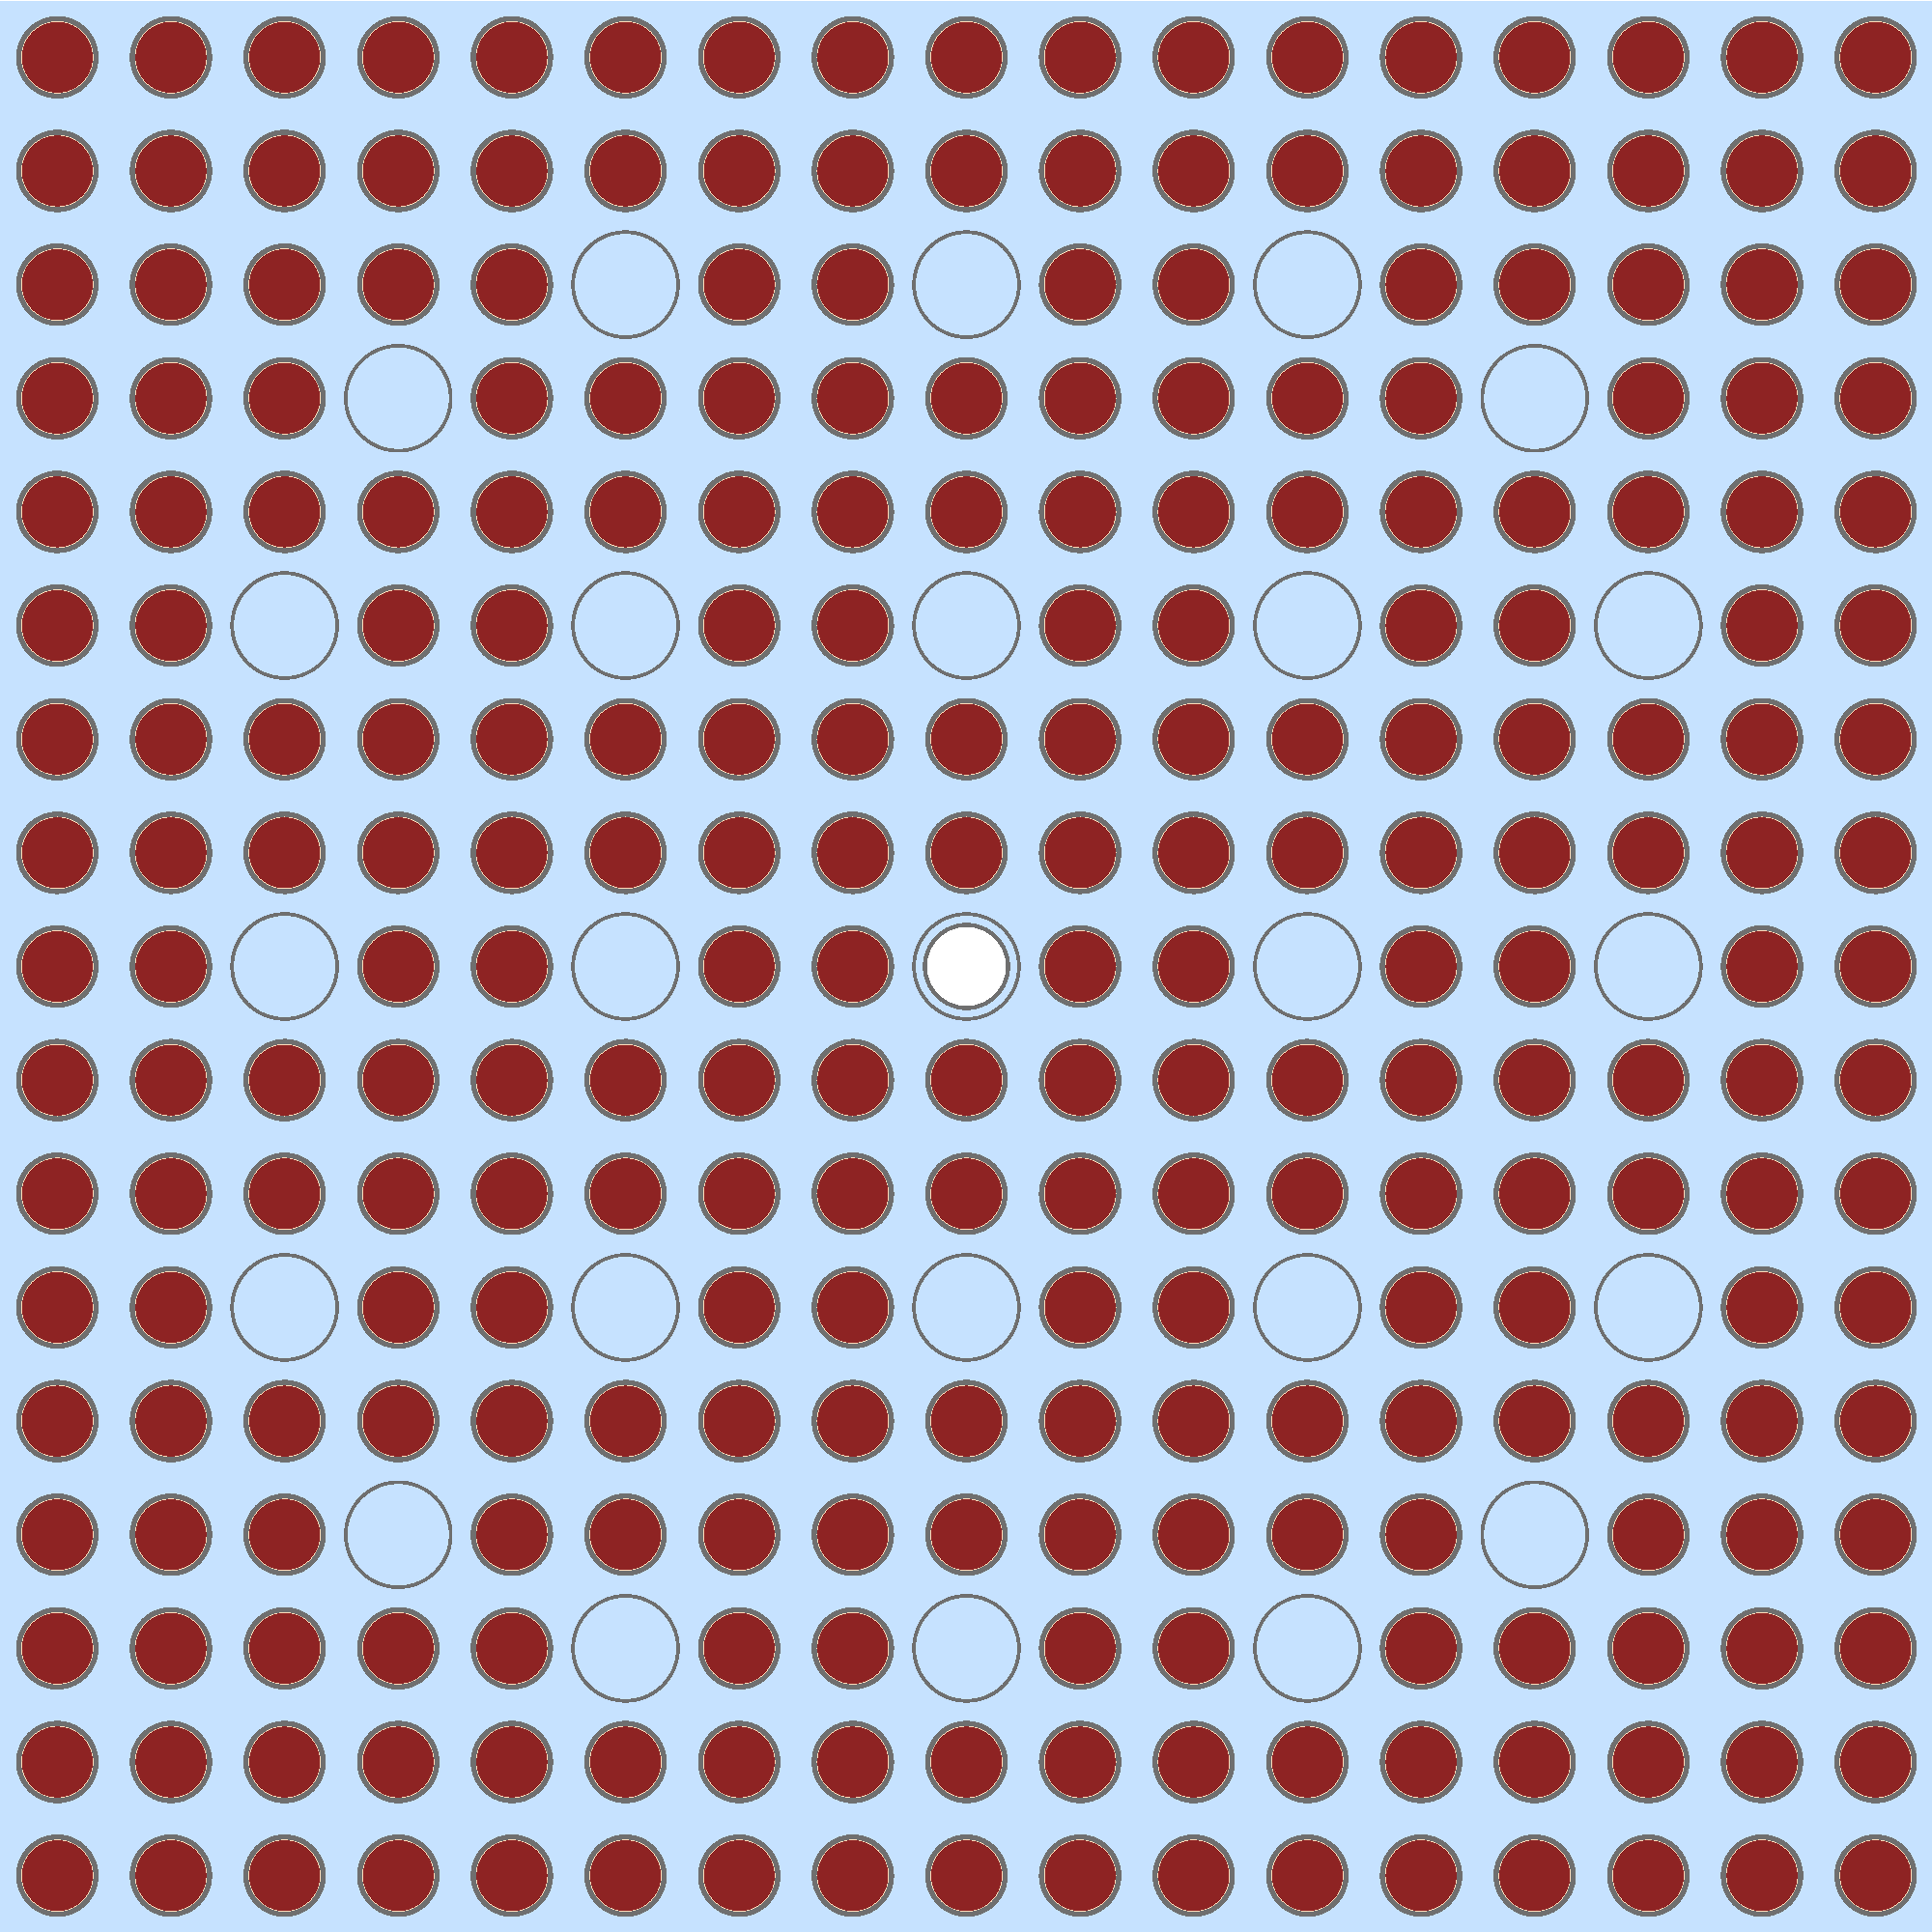
\includegraphics[width=0.8\linewidth]{figures/assembly/geometry}
  \caption{}
  \label{fig:null-assm}
\end{subfigure}
\begin{subfigure}{0.45\textwidth}
  \centering
  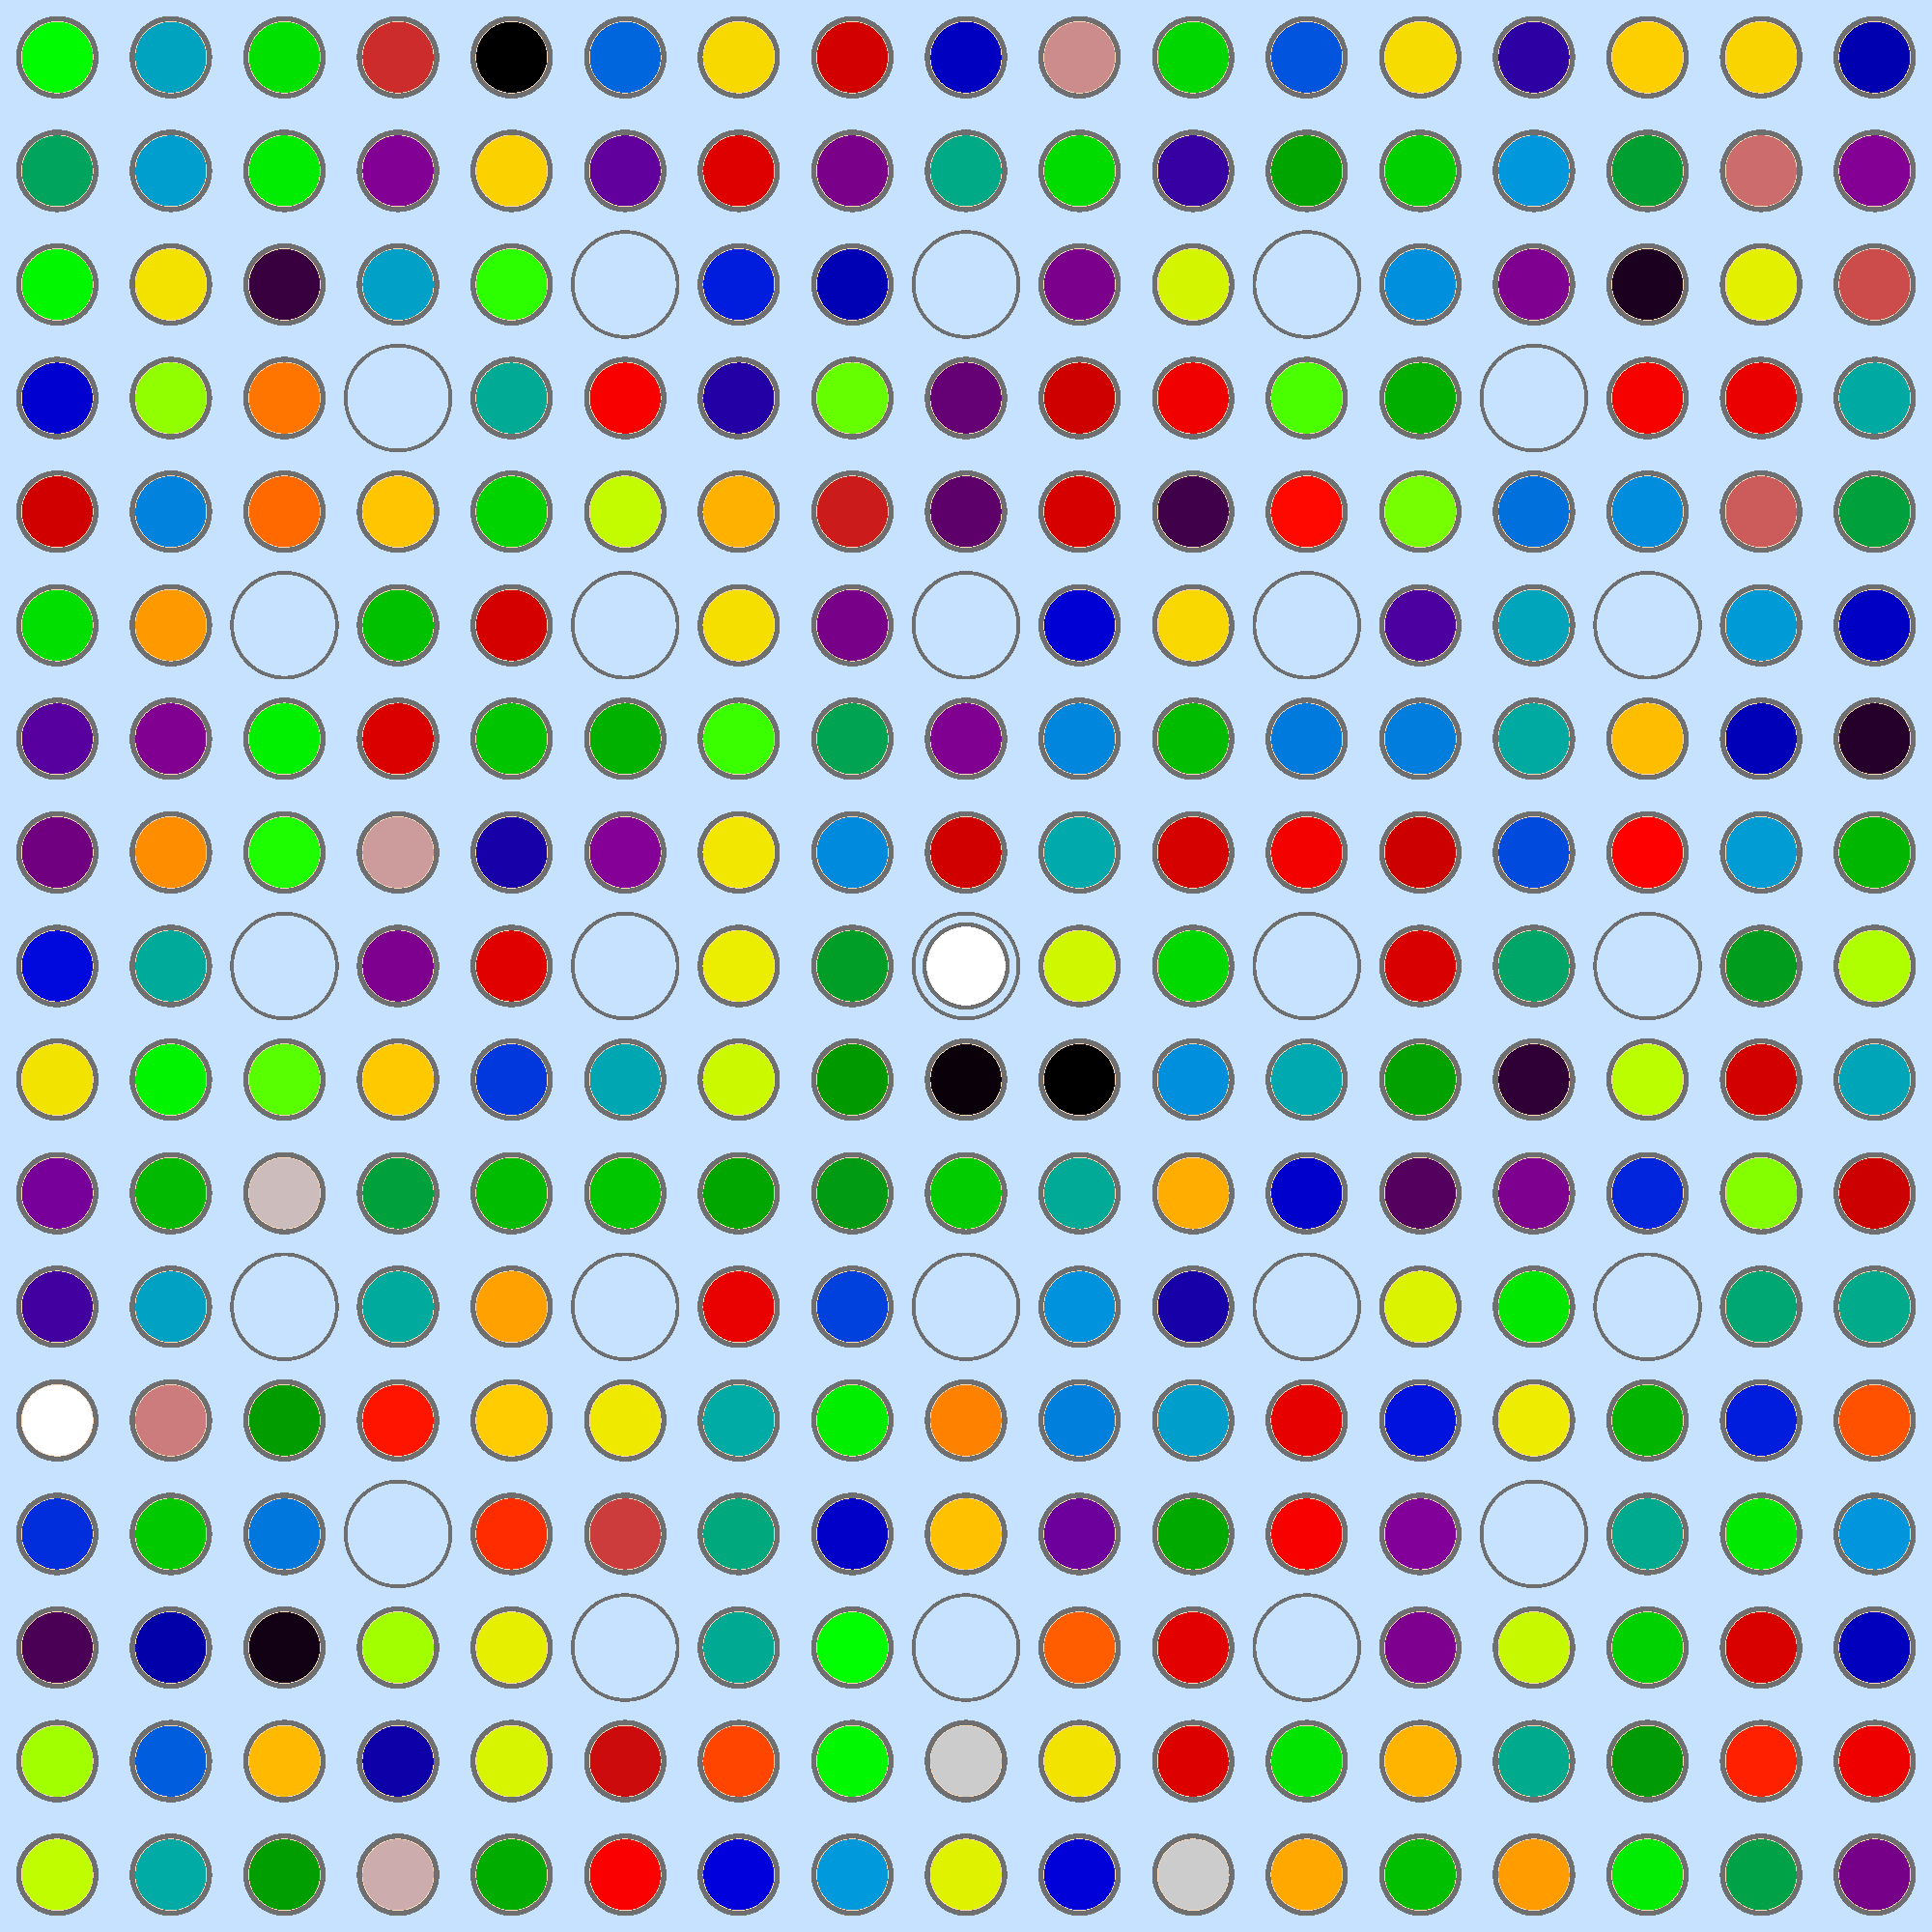
\includegraphics[width=0.8\linewidth]{figures/assembly/degenerate-materials}
  \caption{}
  \label{fig:degenerate-assm}
\end{subfigure}
\begin{subfigure}{0.45\textwidth}
  \centering
  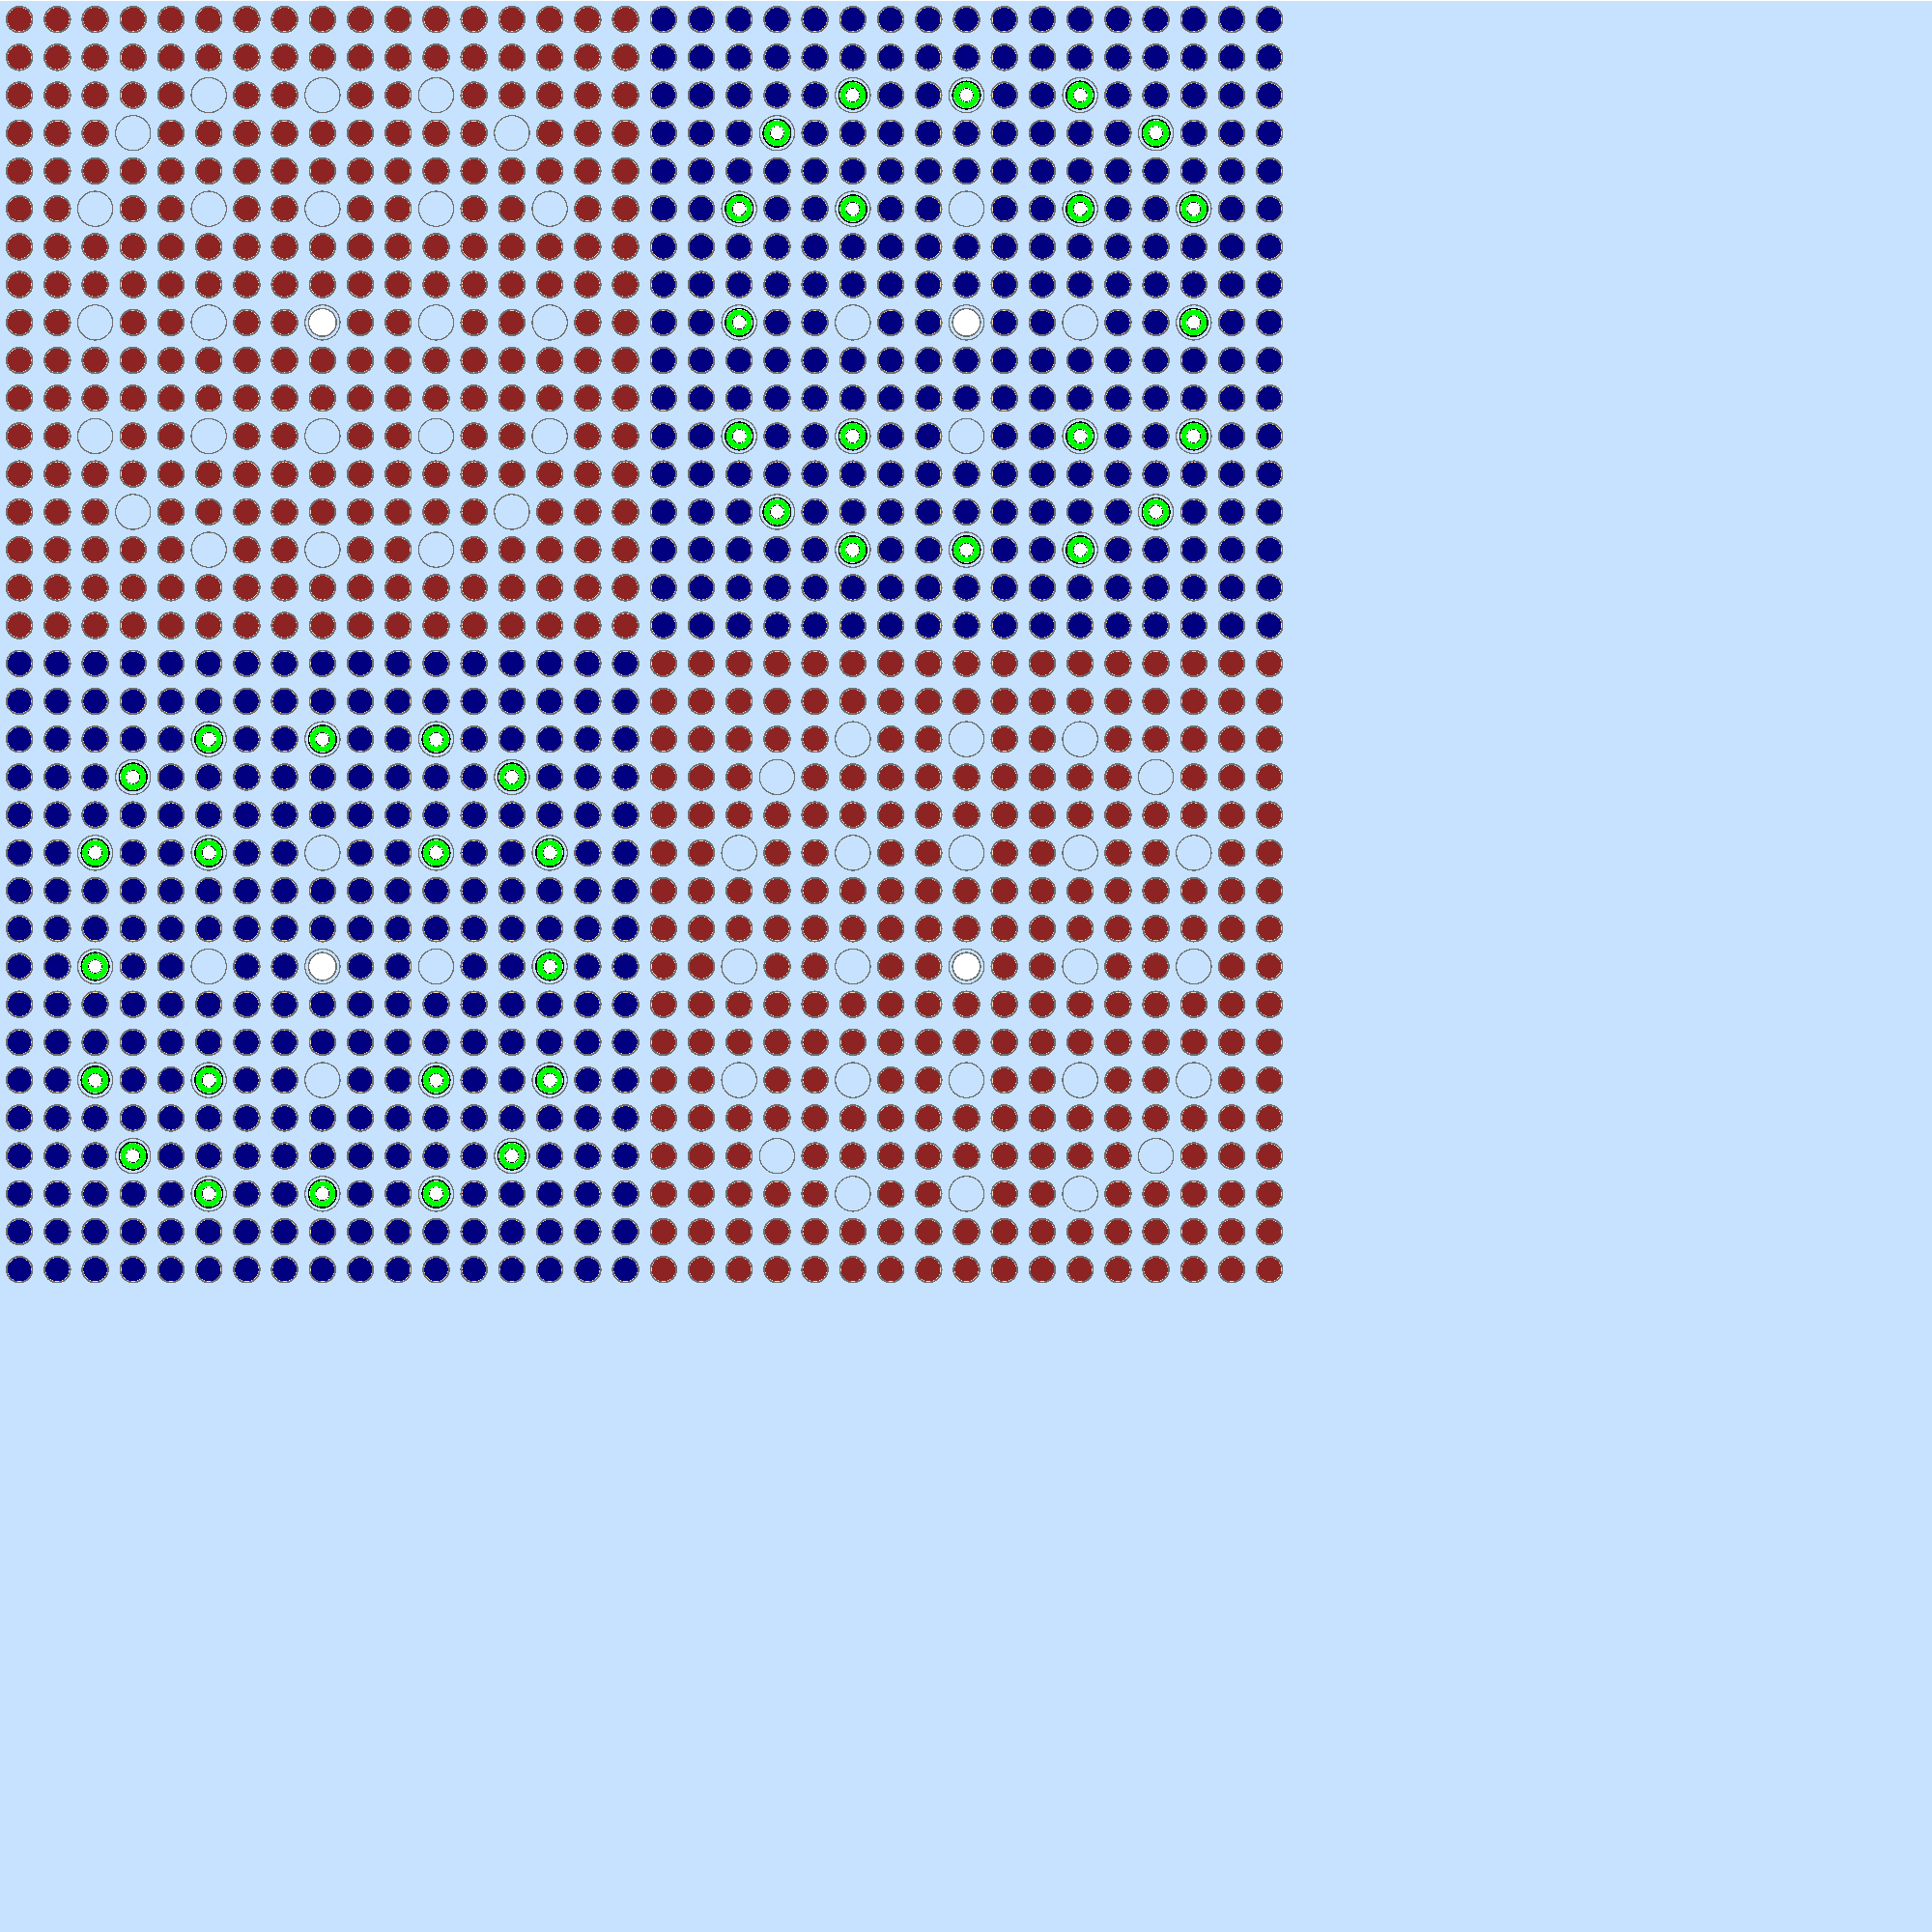
\includegraphics[width=0.8\linewidth]{figures/reflector/geometry}
  \caption{}
  \label{fig:null-reflector}
\end{subfigure}
\begin{subfigure}{0.45\textwidth}
  \centering
  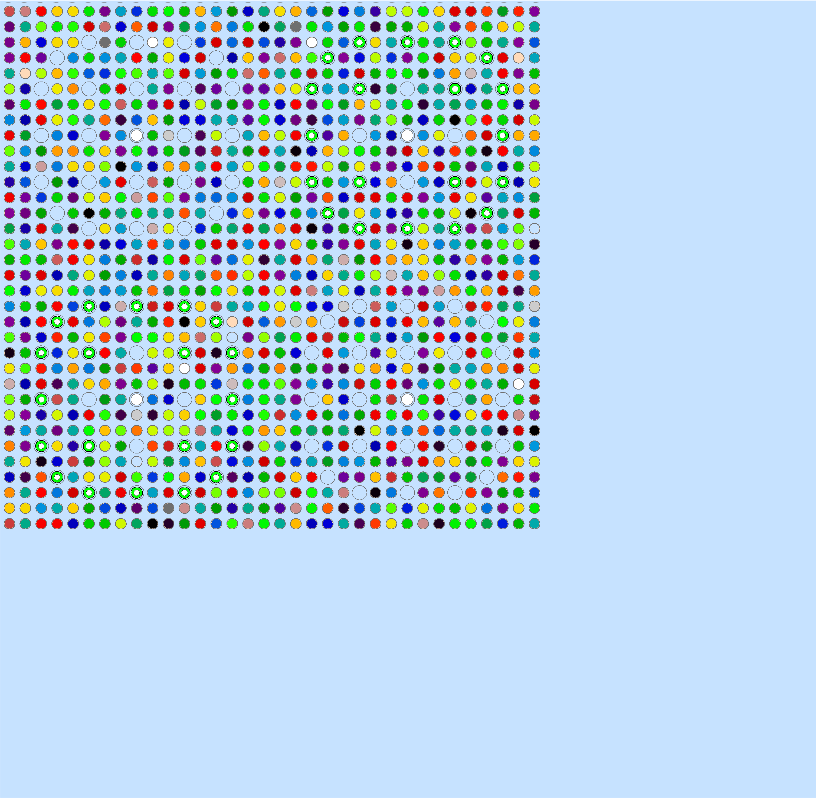
\includegraphics[width=0.8\linewidth]{figures/reflector/degenerate-materials}
  \caption{}
  \label{fig:degenerate-reflector}
\end{subfigure}
\caption{OpenMOC materials for the (a)-(b) assembly and (c)-(d) 2$\times$2 colorset models with null and degenerate homogenization, respectively.}
\label{fig:homogenization-schemes}
\end{figure*}

The \texttt{openmc.mgxs} module was used to compute 70-group MGXS with OpenMC for both the assembly and colorset benchmarks. The tallied MGXS data was condensed to coarse 2-group and 8-group structures with downstream data processing as necessary. The OpenMC simulations were performed with 1000 batches with 10$^{6}$ particle histories per batch for each benchmark. Stationarity of the fission source was obtained with 100 inactive batches for each benchmark. OpenMC's ``iso-in-lab'' feature was employed to enable consistent comparisons between OpenMC's reference results and OpenMOC's calculations with an isotropic in lab scattering source.

%%%%%%%%%%%%%%%%%%%%%%%%%%%%%%%%%%%%%%%%%%%%%%%%%%%%%%%%%%%%%%%%%%%%%%%%%%%%%%%
\subsubsection{Null Homogenization}
\label{subsubsec:homogenize-null}

The \textit{null} spatial homogenization scheme uses a single Monte Carlo calculation of the complete heterogeneous geometry to generate MGXS for each material. In this way, the null scheme fully abandons the multi-level approach used by most traditional approaches to generate MGXS. The spatially self-shielded flux is used to collapse the cross sections in each material with a unique isotopic composition. The null scheme does not account for spatial self-shielding effects experienced by different fuel pins filled by the same type of fuel, and instead averages these effects across the entire geometry. A single MGXS is employed in each instance of a material zone, such as a fuel pin replicated many times throughout a benchmark geometry.

%%%%%%%%%%%%%%%%%%%%%%%%%%%%%%%%%%%%%%%%%%%%%%%%%%%%%%%%%%%%%%%%%%%%%%%%%%%%%%%
\subsubsection{Degenerate Homogenization}
\label{subsubsec:homogenize-degenerate}

Unlike the null spatial homogenization scheme, the \textit{degenerate} scheme accounts for the different spatial self-shielding effects experienced by each instance of each fuel pin throughout a heterogeneous geometry. Like the null scheme, a single MC calculation of the complete heterogeneous geometry is used to generate MGXS for all materials. Unlike the null scheme, the MGXS are tallied separately for each instance of fissile material zones. For example, if a heterogeneous benchmark includes $N$ fuel pins, then $N$ collections of MGXS are separately tabulated for each fuel pin instance. The degenerate scheme tallies different MGXS even if the isotopic compositions in the fuel pin instances are identical (\textit{e.g.}, fresh fuel at the beginning of life) since each instance may experience different spatial self-shielding effects and hence have different MGXS.

The degenerate scheme generates MGXS for each fuel pin instance using OpenMC's distributed cell tallies~\citep{lax2014distribcell}. The OpenCG region differentiation algorithm~\citep{boyd2015opencg} is used to build a new OpenMOC geometry with unique cells and materials for each fuel pin. The MGXS are appropriately selected from OpenMC's distributed cell tallies to populate the MGXS in the OpenMOC materials. Multi-group transport calculations with MGXS generated using null and degenerate schemes may be compared to quantify the impact of modeling spatial self-shielding effects in MGXS for fissile zones in heterogeneous geometries.
%%%%%%%%%%%%%%%%%%%%%%%%%%%%%%%%%%%%%%%%%%%%%%%%%%%%%%%%%%%%%%%%%%%%%%%%%%%%%%%
\section{Test Cases and Reference Results}
\label{sec:Test Cases}
%%%%%%%%%%%%%%%%%%%%%%%%%%%%%%%%%%%%%%%%%%%%%%%%%%%%%%%%%%%%%%%%%%%%%%%%%%%%%%%

This paper models two test cases derived from the Benchmark for Evaluation And Validation of Reactor Simulations (BEAVRS) PWR model~\citep{horelik2013beavrs}. Each test case includes heterogeneous features -- and corresponding spatial self-shielding effects -- in order to understand their implications for accurate pin-wise MGXS generation. Although BEAVRS is an axially heterogeneous 3D core model, both benchmarks were fabricated in 2D due to the geometric constraints in OpenMOC. The impact of fuel enrichment, CRGTs, BPs, inter-assembly currents and water reflectors is considered. The geometric and material specifications for the two test cases are summarized in~\autoref{subsec:benchmarks}. The reference results computed with OpenMC for each of the test cases are discussed in~\autoref{subsec:metrics}.


%%%%%%%%%%%%%%%%%%%%%%%%%%%%%%%%%%%%%%%%%%%%%%%%%%%%%%%%%%%%%%%%%%%%%%%%%%%%%%%
\subsection{Benchmark Configurations}
\label{subsec:benchmarks}

The two test cases were comprised of materials from the BEAVRS model, including 1.6\% and 3.1\% enriched UO$_2$ fuel, borated water\footnote{The water consisted of 975 parts per million (ppm) boron.}, zircaloy, helium, air, borosilicate glass and stainless steel. The densities and isotopic compositions for each material are detailed in the BEAVRS specifications~\citep{horelik2013beavrs}. Each material was modeled with cross sections from the ENDF/B-VII.1 continuous energy cross section library~\citep{mcnpx2003manual} evaluated at 600K for hot zero power conditions.

The first benchmark was a single fuel assembly with an array of 264 fuel pins of 1.6\% enriched UO$_2$ fuel with zircaloy cladding and a helium gap as illustrated in~\autoref{fig:benchmarks-assm}. The assembly included 24 CRGTs of borated water surrounded by zircaloy cladding, and a central instrument tube filled with air surrounded by two zircaloy tubes separated by borated water. The intra-pin egg-crate grid spacer and grid sleeve separating each assembly in the BEAVRS model were not included in the assembly benchmark. The assembly was modeled with reflective boundary conditions.

The second benchmark was constructed as a 2$\times$2 colorset of two fuel assemblies extracted from the BEAVRS model. The top-left and bottom-right fuel assemblies in the colorset were of the same enrichment and configuration as the first benchmark configuration. The top-right and bottom-left fuel assemblies included 264 fuel pins of 3.1\% enriched UO$_2$ fuel, 20 CRGTs and a central instrument tube. In addition, the two 3.1\% enriched assemblies included four BPs consisting of eight layers of air, steel, borosilicate glass and zircaloy. The colorset was surrounded by a water reflector on the bottom and right that was of the same width as a fuel assembly. The reflected colorset included reflective boundaries on the top and left (adjacent to the fuel assemblies) with vacuum boundaries on the bottom and right (adjacent to the reflector).

%The colorset does not include the stainless steel baffle surrounding the fuel assemblies adjacent to the water reflector in the full core BEAVRS model.

\begin{figure}[ht!]
\centering
\begin{subfigure}{0.45\textwidth}
  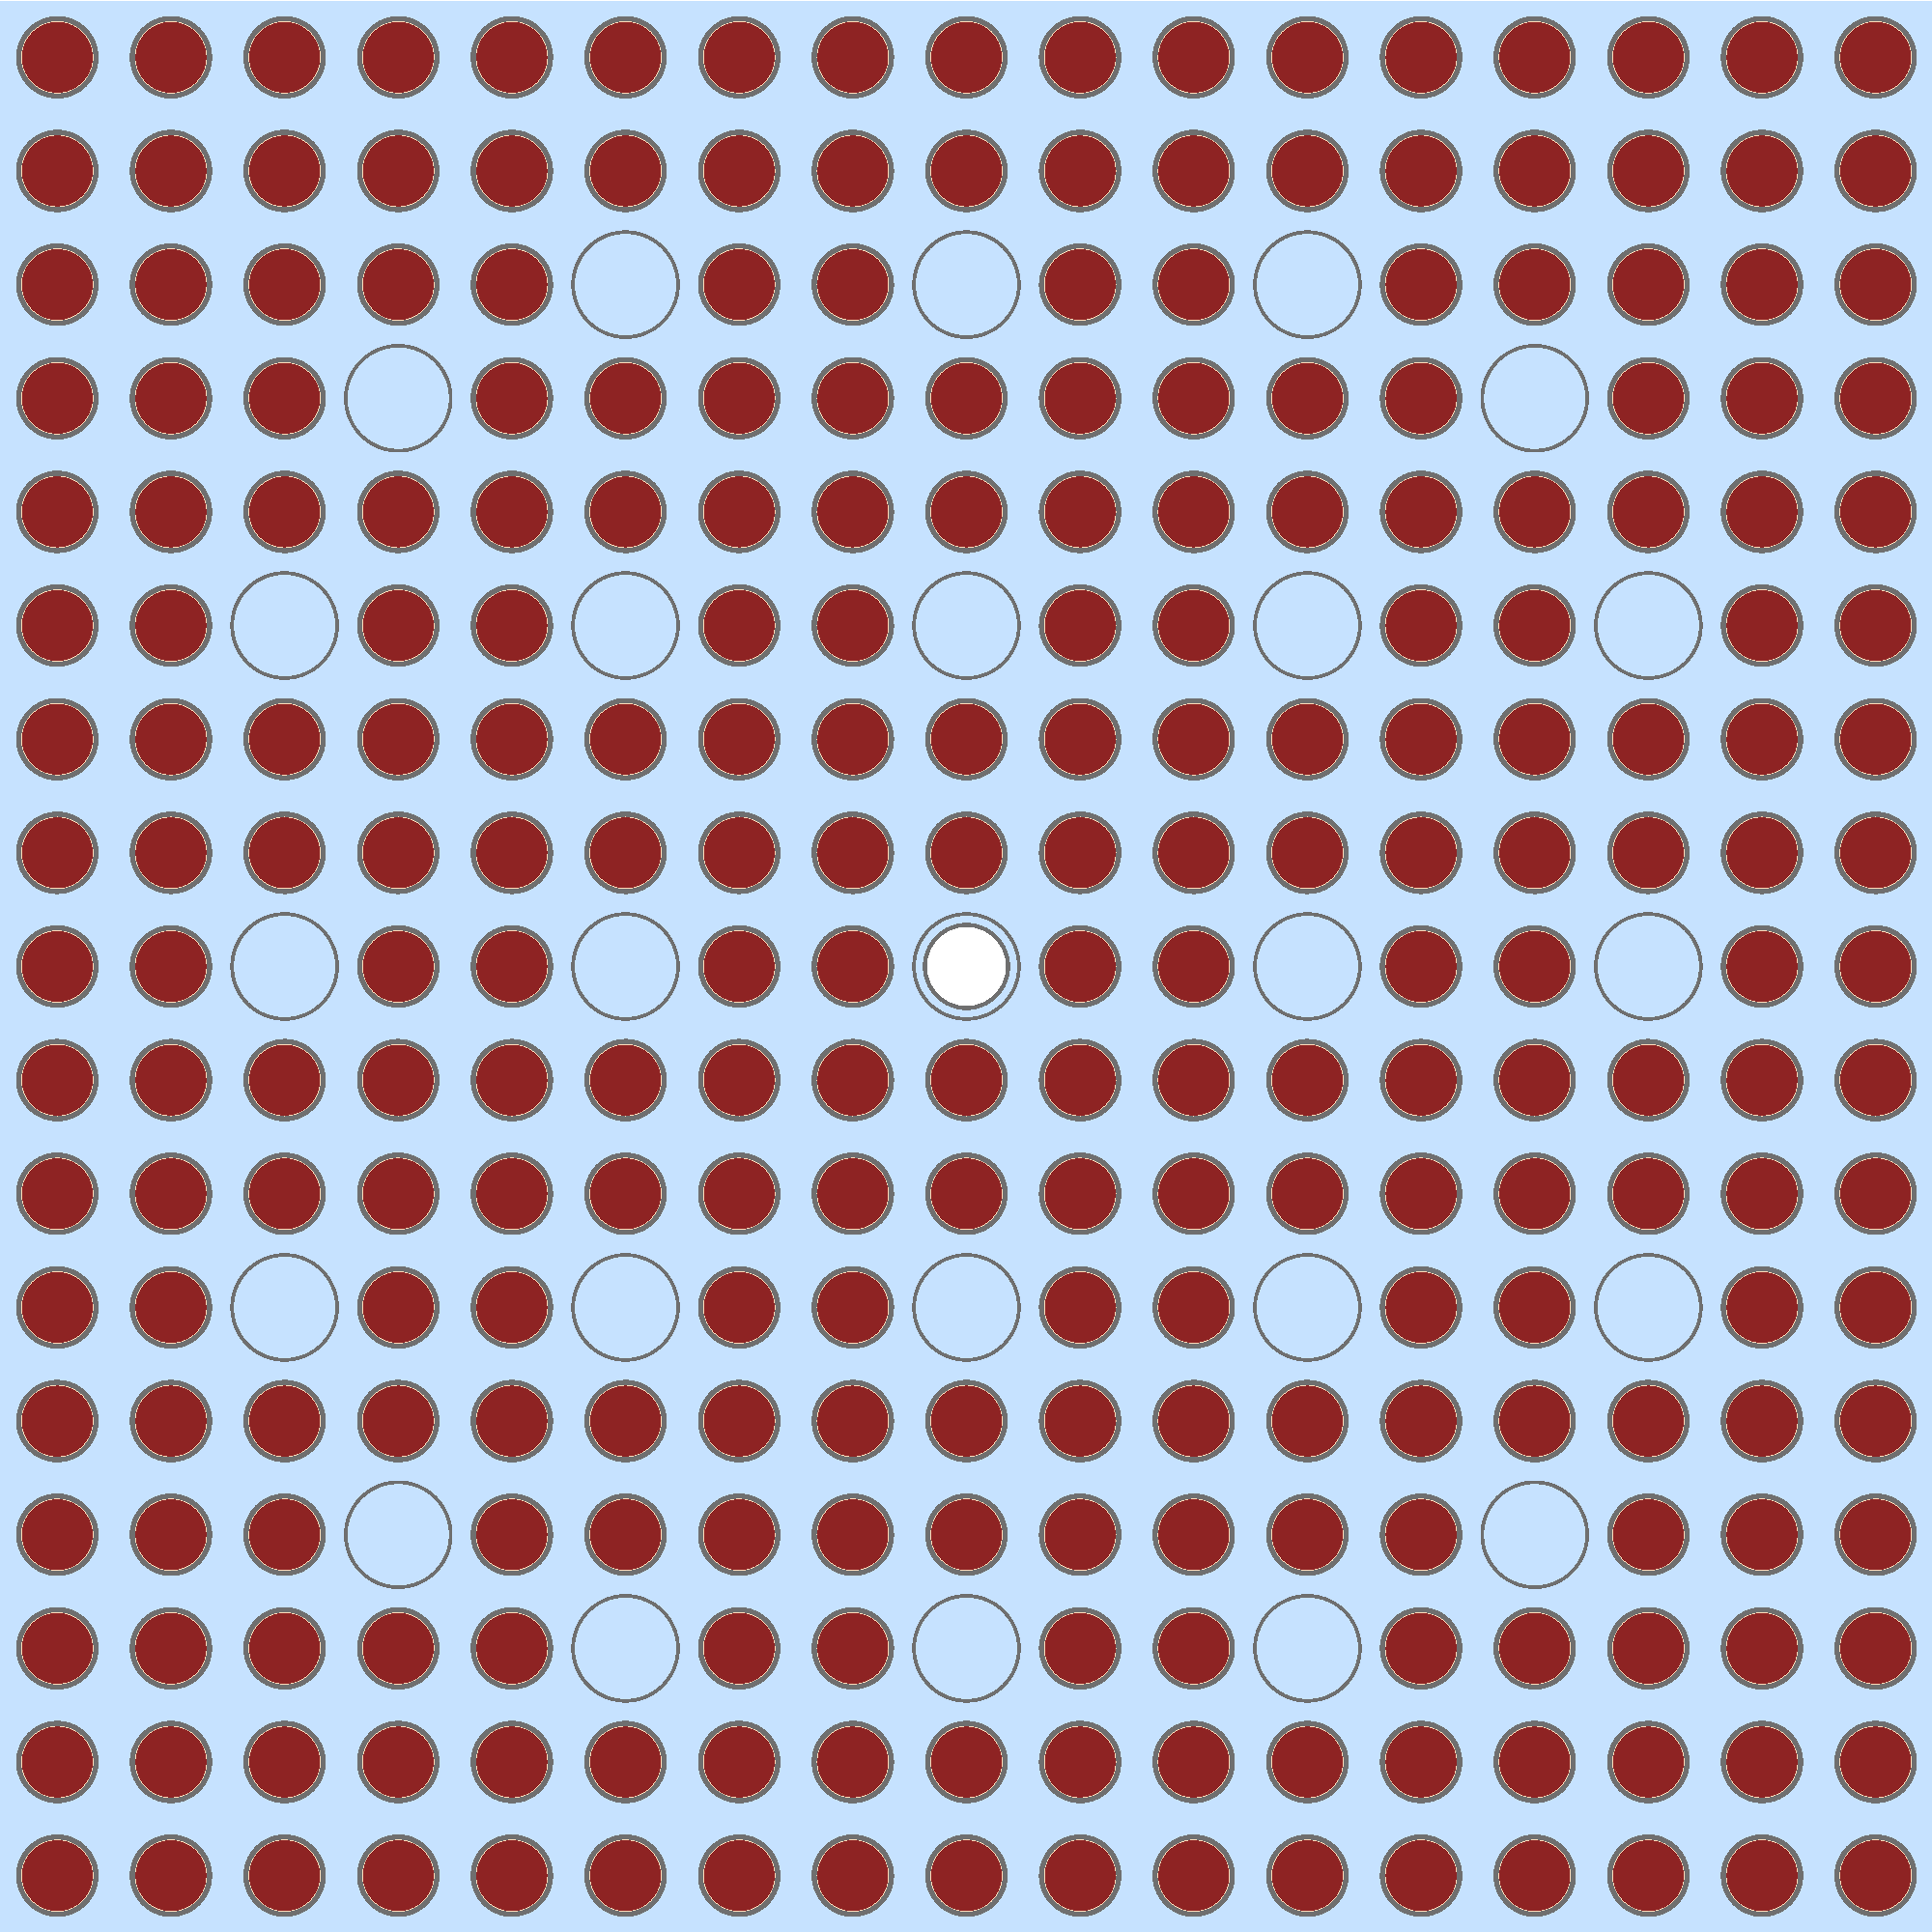
\includegraphics[width=\linewidth]{figures/assembly/geometry}
  \caption{}
  \label{fig:benchmarks-assm}
\end{subfigure}
\begin{subfigure}{0.45\textwidth}
  \centering
  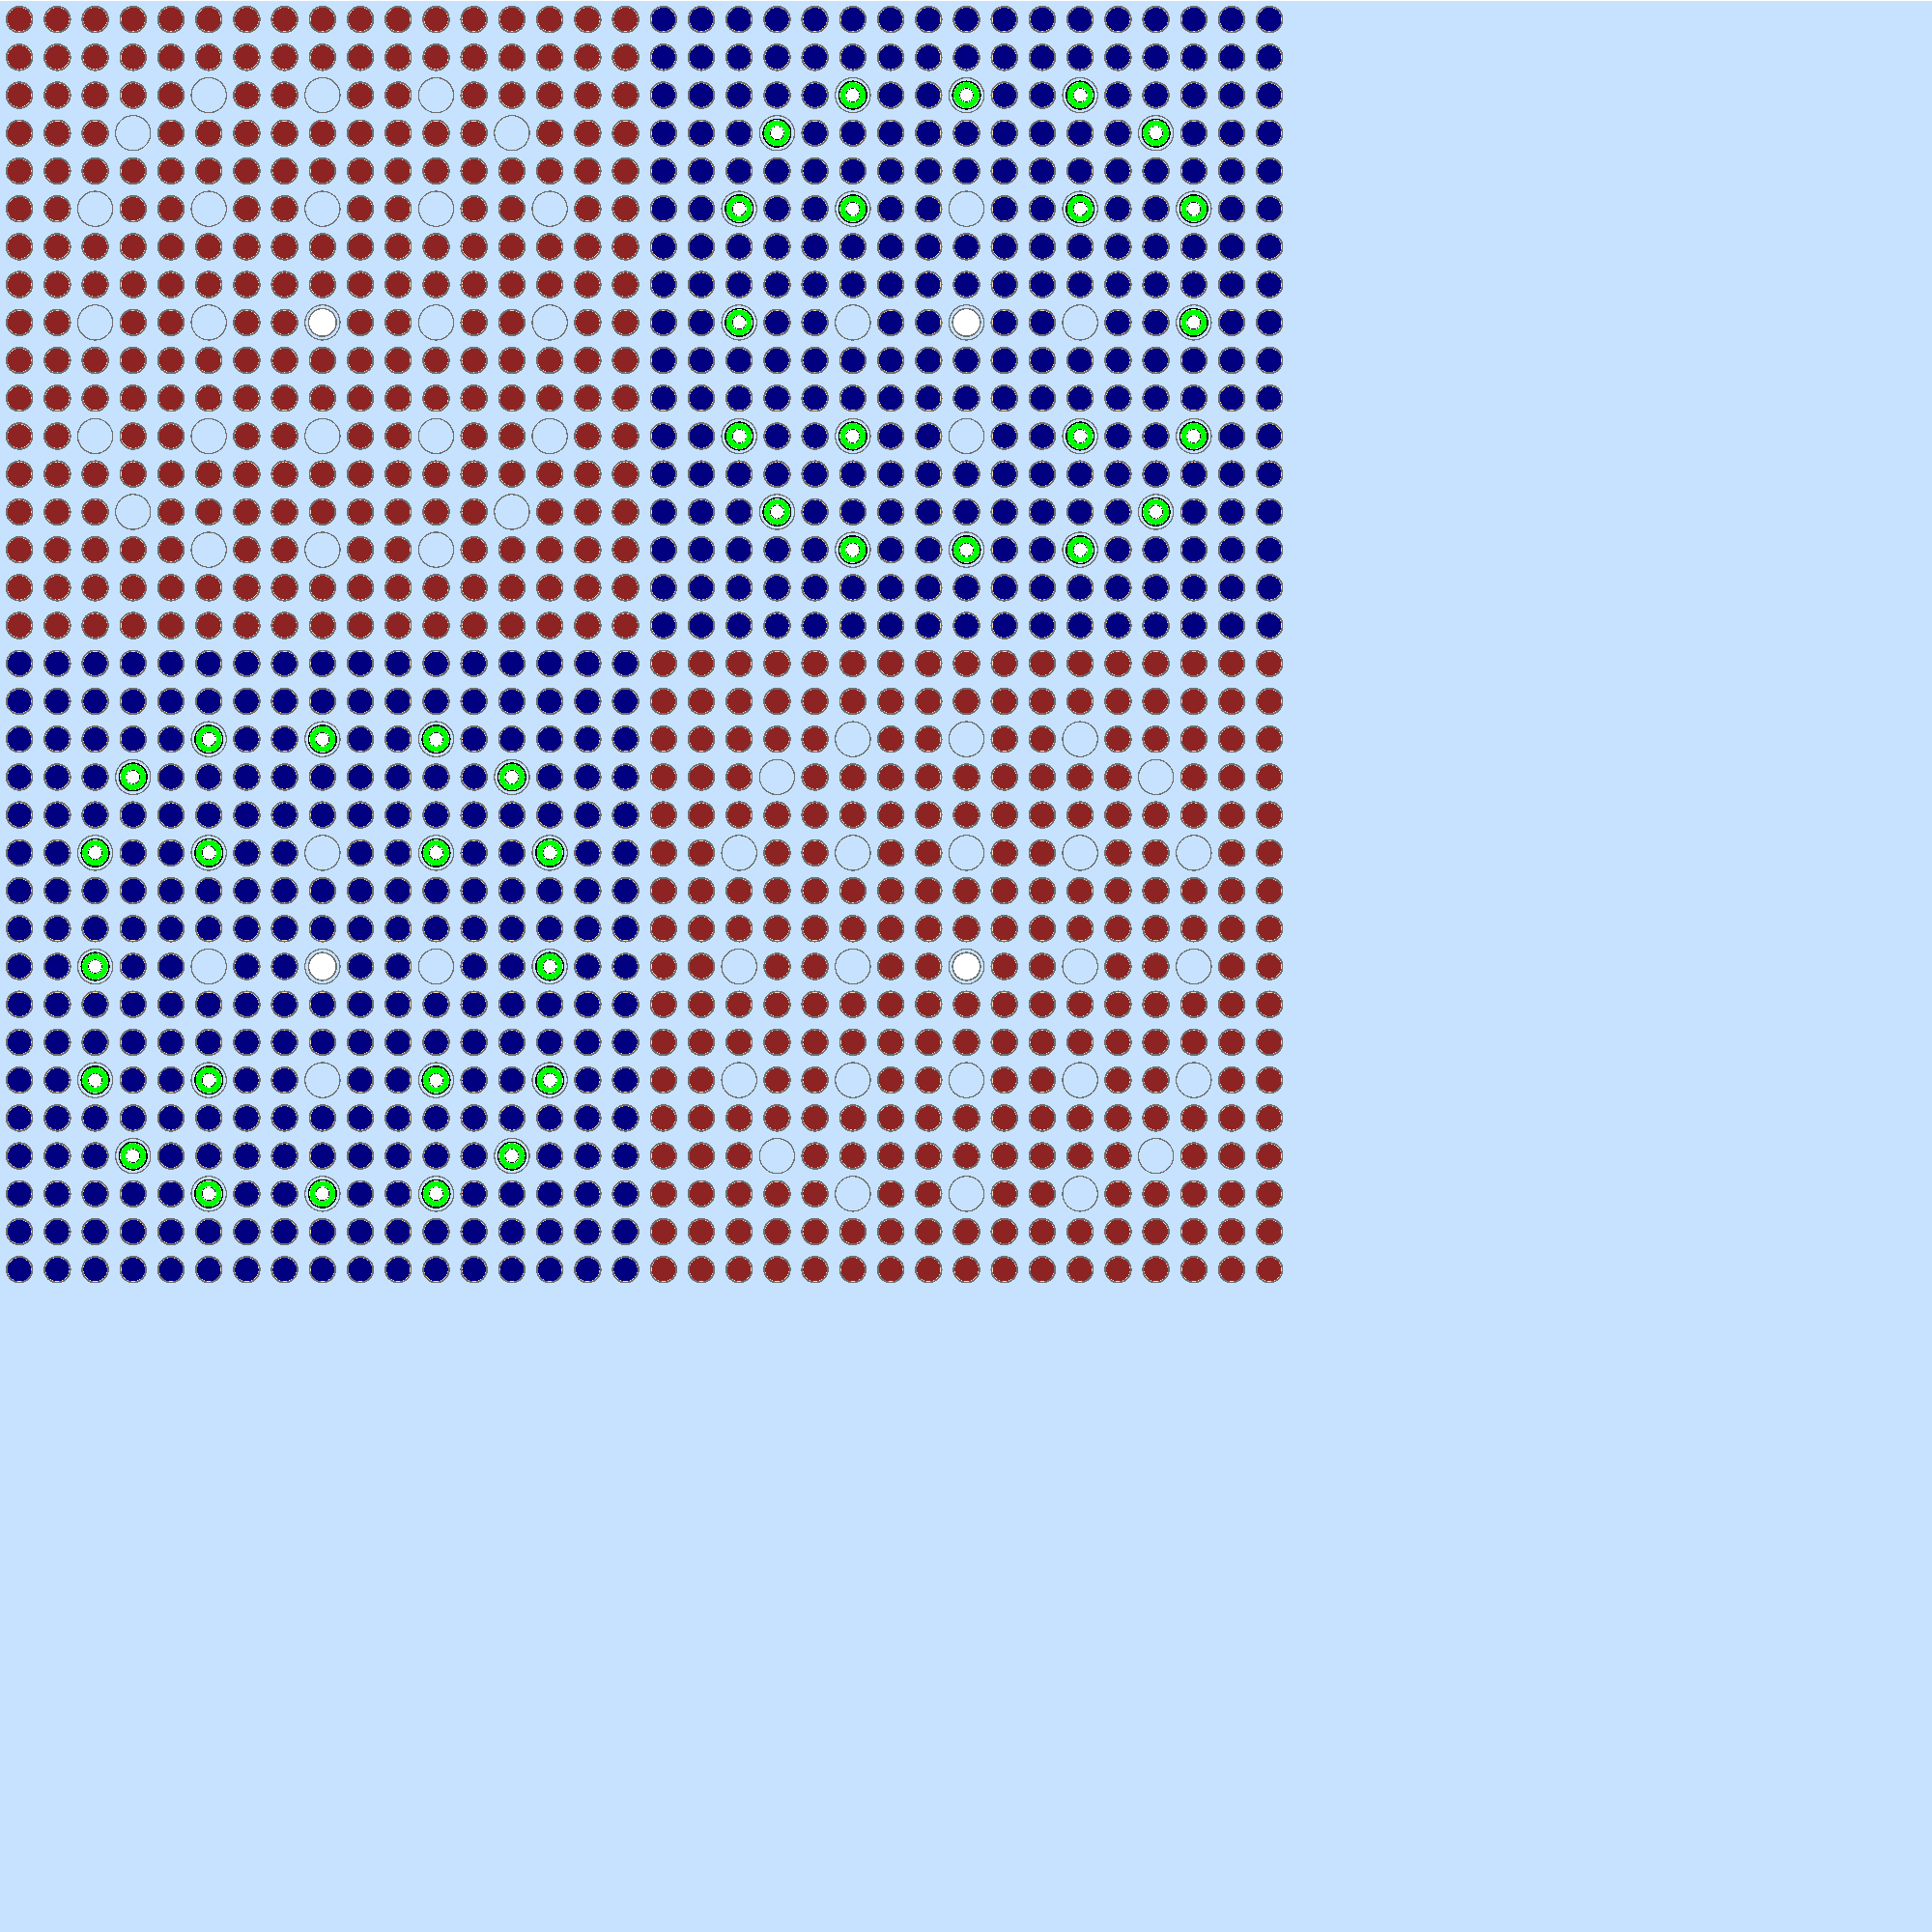
\includegraphics[width=\linewidth]{figures/reflector/geometry}
  \caption{}
  \label{fig:benchmarks-reflector}
\end{subfigure}
\caption{A (a) fuel assembly and (b) 2$\times$2 assembly colorset with reflector.}
\label{fig:benchmarks}
\end{figure}


%%%%%%%%%%%%%%%%%%%%%%%%%%%%%%%%%%%%%%%%%%%%%%%%%%%%%%%%%%%%%%%%%%%%%%%%%%%%%%%
\subsection{Verification Metrics}
\label{subsec:metrics}

A series of OpenMC simulations were used to calculate reference eigenvalues, pin-wise fission rates, and pin-wise U-238 capture rates for both benchmarks. The reference solutions were computed with 100 inactive and 900 active batches of 10$^7$ particle histories per batch. It should be noted that isotropic in lab scattering was employed for all reference calculations with OpenMC's ``iso-in-lab'' feature\footnote{The OpenMC ``iso-in-lab'' feature samples the outgoing neutron energy from the scattering laws prescribed by the continuous energy cross section library, but the outgoing neutron direction of motion is sampled from an isotropic in lab distribution.}. Although isotropic in lab scattering is a poor approximation for LWRs, it eliminated scattering source anisotropy as one possible cause of approximation error between OpenMC and OpenMOC in order to isolate approximation errors resulting from spatially self-shielded MGXS.

The reference eigenvalues are listed in~\autoref{tab:keff-reference}. The OpenMC ``combined'' eigenvalue estimator is reported along with the associated 1-sigma uncertainty of one pcm for both test cases.

\begin{table}[h!]
  \centering
  \caption{Reference OpenMC eigenvalues for each test case.}
  \label{tab:keff-reference} 
  \begin{tabular}{c c}
  \toprule
  {\bf Assembly} &
  {\bf Colorset} \\
  \midrule
  0.99326 $\pm$ 0.00001 & 0.94574 $\pm$ 0.00001 \\
  \bottomrule
\end{tabular}
\end{table}

The reference energy-integrated fission and U-238 capture rate spatial distributions were computed using rectilinear, pin-wise tally meshes in OpenMC and are shown in~\autoref{fig:fiss-capt-rates}. The reaction rates were volume-integrated across each fuel pin. The fission rates include fission from only U-235 and U-238 for the fresh PWR UO$_2$ fuel. The reaction rates were normalized to the mean of all non-zero reaction rates in each benchmark. The reaction rates in the instrument tubes, CRGTs and BPs are all zero and are illustrated in white. The 1-sigma uncertainties are less than 0.08\% in each pin for each benchmark.

\begin{figure*}[h!]
\centering
\begin{subfigure}{0.45\textwidth}
  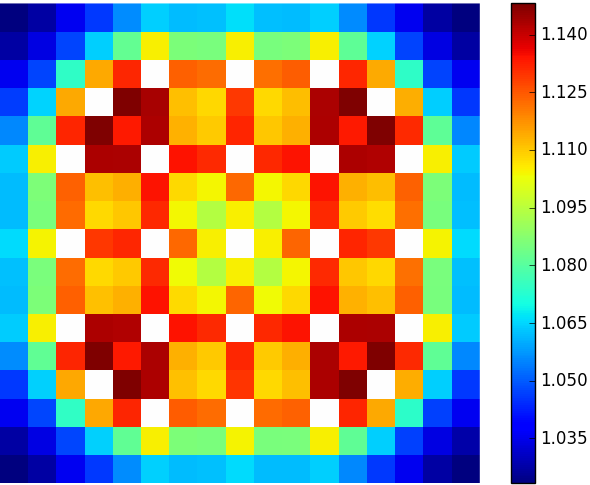
\includegraphics[width=\linewidth]{figures/assembly/fission-rates}
  \caption{}
  \label{fig:fiss-assm}
\end{subfigure}%
\begin{subfigure}{0.45\textwidth}
  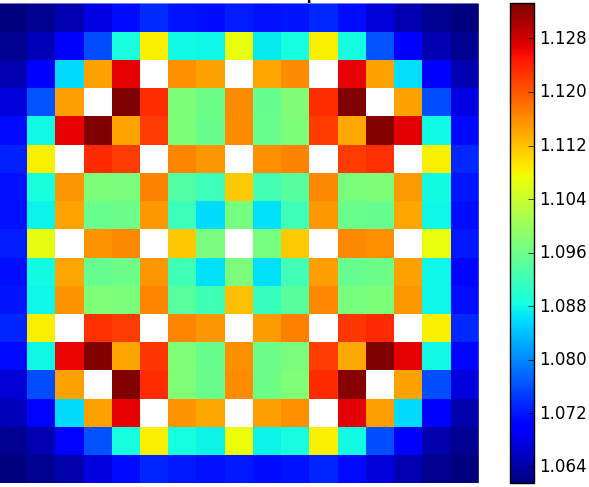
\includegraphics[width=\linewidth]{figures/assembly/capture-rates}
  \caption{}
  \label{fig:capt-assm}
\end{subfigure}
\begin{subfigure}{0.45\textwidth}
  \centering
  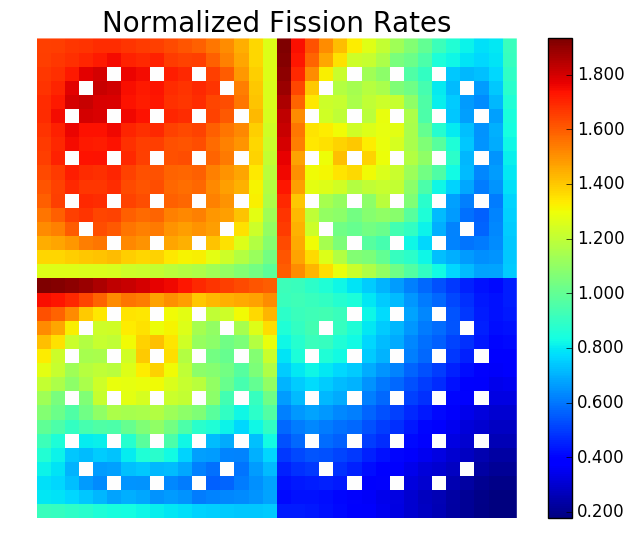
\includegraphics[width=\linewidth]{figures/reflector/fission-rates}
  \caption{}
  \label{fig:fiss-reflector}
\end{subfigure}%
\begin{subfigure}{0.45\textwidth}
  \centering
  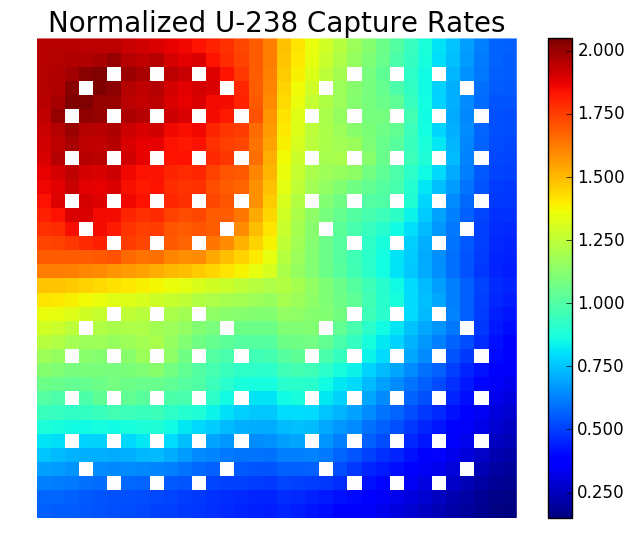
\includegraphics[width=\linewidth]{figures/reflector/capture-rates}
  \caption{}
  \label{fig:capt-reflector}
\end{subfigure}
\caption{Fission and U-238 capture rates for the (a) -- (b) assembly and (c) -- (d) colorset.}
\label{fig:fiss-capt-rates}
\end{figure*}

As illustrated in the figures, the reaction rate rate distributions are strongly dependent on the spatially heterogeneous features in each benchmark. For example, the CRGTs provide additional moderation and increase the fision and U-238 capture rates in nearby fuel pins. The inclusion of BPs reduces the neutron population and therefore the reaction rates for the surrounding fuel pins. The presence of a reflector with a mixture of vacuum and reflective BCs induces a tilt in the reaction rates across the assemblies in the colorset.

Although spatial heterogeneities generally have similar effects on both fission and U-238 capture rates, there are a few important differences to note. The U-238 capture rates in the assemblies are more sensitive than the fission rates to the spatial self-shielding induced by moderation in CRGTs. In addition, the capture rates in the colorset are more smoothly varying at the inter-assembly and assembly-reflector interfacea than the fission rates.
%%%%%%%%%%%%%%%%%%%%%%%%%%%%%%%%%%%%%%%%%%%%%%%%%%%%%%%%%%%%%%%%%%%%%%%%%%%%%%%
\section{Results}
\label{sec:results}
%%%%%%%%%%%%%%%%%%%%%%%%%%%%%%%%%%%%%%%%%%%%%%%%%%%%%%%%%%%%%%%%%%%%%%%%%%%%%%%

Both benchmarks were modeled with OpenMOC using MGXS generated by OpenMC for the null, degenerate and LNS spatial homogenization schemes. The eigenvalues and pin-wise fission and U-238 capture rates computed by OpenMOC are compared to the reference OpenMC solutions in \autoref{subsec:eigenvalues}, \autoref{subsec:fiss-rates} and \autoref{subsec:capt-rates}, respectively.


%%%%%%%%%%%%%%%%%%%%%%%%%%%%%%%%%%%%%%%%%%%%%%%%%%%%%%%%%%%%%%%%%%%%%%%%%%%%%%%
\subsection{Eigenvalues}
\label{subsec:eigenvalues}

The OpenMOC eigenvalues were compared to the reference OpenMC eigenvalues from \autoref{tab:keff-reference}. The eigenvalue bias $\Delta\rho$ was calculated by comparing the eigenvalue $k_{eff}^{MOC}$ from OpenMOC to the reference eigenvalue $k_{eff}^{MC}$ computed by OpenMC in units of per cent mille (pcm):

\begin{equation}
\label{eqn:delta-rho}
\Delta\rho = \left(k_{eff}^{MOC} - k_{eff}^{MC}\right) \times 10^{5}
\end{equation}

The bias is listed for both benchmarks and the three spatial homogenization schemes in \autoref{tab:keff-bias}. The slightly negative bias of a few hundred pcm is likely due to the flux separability approximation \citep{boyd2018sph}, which permits use of the scalar rather than the angular neutron flux to collapse cross sections. The eigenvalues for the three schemes are identical for the fuel assembly and are consistent to within 10 pcm for the colorset benchmark. As these results show, the choice of spatial homogenization scheme is inconsequential to the eigenvalue predictions. This is to be expected since the three methods use the same MC flux to collapse the MGXS and preserve global reactivity.

%It should be recalled that isotropic in lab scattering is used by OpenMC to compute both the reference solution and the MGXS. If anisotropic scattering were employed in OpenMC, one would expect quite different biases without a robust implementation of a higher order scattering kernel in OpenMOC.

\begin{table}[h!]
  \centering
  \caption{OpenMOC eigenvalue bias $\Delta\rho$.}
  \label{tab:keff-bias}
  \begin{tabular}{l c c c}
  \toprule
  \textbf{Benchmark} & \textbf{Null} & \textbf{Degenerate} & \textbf{LNS} \\
  \midrule
  Assembly & -161 & -161 & -161 \\
  Colorset & -142 & -132 & -138 \\
  \bottomrule
\end{tabular}
\end{table}


%%%%%%%%%%%%%%%%%%%%%%%%%%%%%%%%%%%%%%%%%%%%%%%%%%%%%%%%%%%%%%%%%%%%%%%%%%%%%%%
\subsection{Fission Rates}
\label{subsec:fiss-rates}

The OpenMOC energy-integrated pin-wise fission rates were compared to the reference OpenMC fission rates shown in \autoref{fig:fiss-assm} and \autoref{fig:fiss-reflector}. The percent relative errors for each pin's fission rates were computed and the maximum and mean errors are listed for both benchmarks and the three spatial homogenization schemes in \autoref{tab:fiss-errors}. In particular, the maximum errors are the maximum of the absolute values of the errors along with the appropriate sign, while the mean errors are the averages of the absolute error magnitudes. The fission rate errors are somewhat dependent on the spatial homogenization scheme used to compute MGXS in the fuel. In particular, the degenerate scheme produces slightly smaller maximum and mean errors than the null scheme.

\begin{table}[h!]
  \centering
  \caption{OpenMOC fission rate percent relative errors.}
  \label{tab:fiss-errors}
  \begin{tabular}{l l r r r}
  \toprule
  \textbf{Benchmark} & \textbf{Metric} & \textbf{Null} & \textbf{Degenerate} & \textbf{LNS} \\
  \midrule
  \multirow{2}{*}{Assembly} & Max  & 0.380 & 0.315 & 0.314 \\
                            & Mean & 0.074 & 0.079 & 0.078 \\
  \midrule
  \multirow{2}{*}{Colorset} & Max  & 0.764 & 0.602 & 0.709 \\
                            & Mean & 0.178 & 0.138 & 0.155 \\
  \bottomrule
\end{tabular}
\end{table}

%The spatial distributions of fission rate errors are plotted as heatmaps for each benchmark in \autoref{fig:fiss-errors}. The heatmaps illustrate systematic trends in the pin-wise fission errors which correlate with spatial heterogeneities in each benchmark. In particular, the fission rates are generally underpredicted for pins adjacent to a single CRGT, but overpredicted for pins adjacent to two CRGTs in the assembly. In addition, the errors are largest for pins along the inter-assembly and assembly-reflector interfaces for the colorset benchmark.

%For the PWR benchmarks modeled here, the moderation provided by neighboring CRGTs and reflectors softens the flux for nearby fuel pins and should be modeled when collapsing pin-wise MGXS for high-fidelity multi-group transport calculations.

% FIXME: Need to either (a) plot fission rate errors for LNS or (b) remove the figure and instead point to the table of errors to say that the difference is small

%\begin{figure*}[h!]
%\centering
%\begin{subfigure}{0.45\textwidth}
%  \centering
%  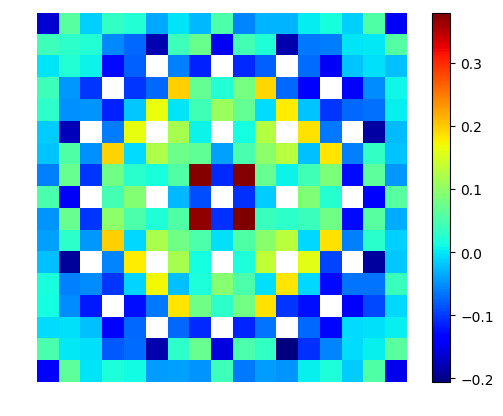
\includegraphics[width=\linewidth]{figures/assembly/fiss-null-errors}
%  \caption{}
%  \label{fig:assm-fiss-null-error}
%\end{subfigure}%
%\begin{subfigure}{0.45\textwidth}
%  \centering
%  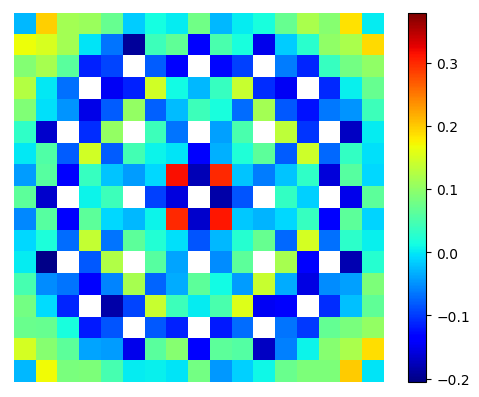
\includegraphics[width=\linewidth]{figures/assembly/fiss-degenerate-errors}
%  \caption{}
%  \label{fig:assm-fiss-degen-error}
%\end{subfigure}
%\begin{subfigure}{0.45\textwidth}
%  \centering
%  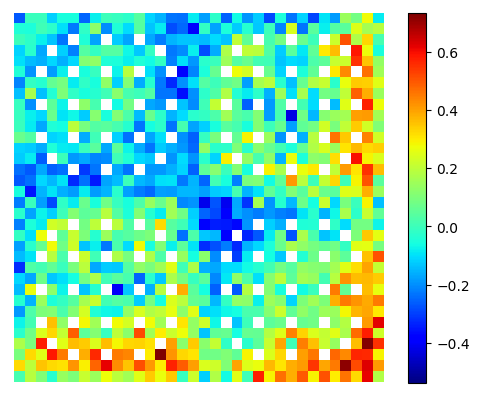
\includegraphics[width=\linewidth]{figures/reflector/fiss-null-errors}
%  \caption{}
%  \label{fig:reflector-fiss-null-error}
%\end{subfigure}%
%\begin{subfigure}{0.45\textwidth}
%  \centering
%  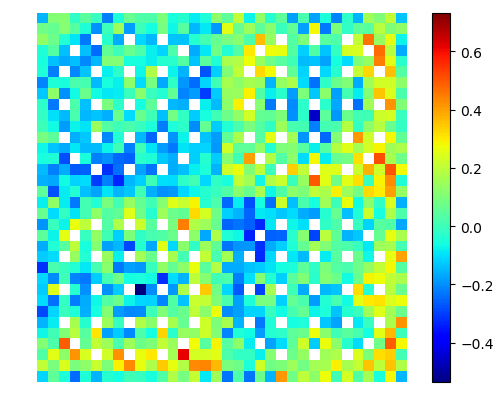
\includegraphics[width=\linewidth]{figures/reflector/fiss-degenerate-errors}
%  \caption{}
%  \label{fig:reflector-fiss-degen-error}
%\end{subfigure}
%\caption{OpenMOC fission rate percent relative errors for the assembly (a) and colorset (b) benchmarks.}
%\label{fig:fiss-errors}
%\end{figure*}


%%%%%%%%%%%%%%%%%%%%%%%%%%%%%%%%%%%%%%%%%%%%%%%%%%%%%%%%%%%%%%%%%%%%%%%%%%%%%%%
\subsection{Capture Rates}
\label{subsec:capt-rates}

The OpenMOC energy-integrated pin-wise U-238 capture rates were compared to the reference OpenMC capture rates shown in \autoref{fig:capt-assm} and \autoref{fig:capt-reflector} for the assembly and reflector, respectively. The percent relative errors for each pin's capture rates were computed and the maximum and mean errors are listed for both benchmarks and the three spatial homogenization schemes in \autoref{tab:capt-errors}. In particular, the maximum errors are the maximum of the absolute values of the errors along with the appropriate sign, while the mean errors are the averages of the absolute error magnitudes.

\begin{table}[h!]
  \centering
  \caption{OpenMOC U-238 capture rate percent relative errors.}
  \label{tab:capt-errors} 
  \begin{tabular}{l l r r r}
  \toprule
  \textbf{Benchmark} & \textbf{Metric} & \textbf{Null} & \textbf{Degenerate} & \textbf{LNS} \\
  \midrule
  \multirow{2}{*}{Assembly} & Max  & -1.101 &  0.386 & 0.290 \\
                            & Mean &  0.479 &  0.086 & 0.076 \\
  \midrule
  \multirow{2}{*}{Colorset} & Max  & -1.969 & -0.783 & -1.964 \\
                            & Mean &  0.478 &  0.165 & 0.236 \\
  \bottomrule
\end{tabular}
\end{table}

The capture rate errors are more dependent on the spatial homogenization scheme used to compute MGXS in the fuel than are the fission rate errors. In particular, the degenerate scheme produces much smaller maximum and mean errors than the null scheme. The maximum error is greater than 1\% for both benchmarks with the null scheme, but is reduced by 2 -- 5$\times$ with the use of degenerate homogenization. This underscores the importance of accounting for spatial heterogeneities when generating MGXS to predict U-238 capture and Pu-239 production in LWRs. The moderation provided by neighboring CRGTs and reflectors softens the flux for nearby fuel pins and should be modeled when collapsing pin-wise MGXS for high-fidelity multi-group transport calculations.

The max and mean U-238 capture rate errors are reduced by 3.7$\times$ and 6.3$\times$, respectively, for LNS with respect to null homogenization for the assembly. This demonstrates that LNS homogenization more accurately models inter-pin spatial self-shielding effects in pin-wise MGXS. Furthermore, the max and mean errors are reduced by 10\% and 25\% relative to degenerate homogenization. This latter observation indicates that LNS de-noises the statistical uncertainties of the MC-generated MGXS by averaging the MGXS for each grouping of fuel pins, resulting in MGXS with smaller uncertainties than those generated by degenerate homogenization. However, the results are significantly different for the colorset. In particular, the max error for the colorset with LNS homogenization is very nearly the same as those for null homogenization. The MGXS for the fuel pins near the assembly-reflector interface are not separately homogenized with LNS and thus fail to account for the additional moderation from the reflector.

The spatial distributions of capture rate errors are plotted as heatmaps for the assembly and colorset in \autoref{fig:assm-capt-errors} and \autoref{fig:reflector-capt-errors}, respectively. The null scheme exhibits the largest errors for pins near CRGTs and along the inter-assembly and assembly-reflector interfaces, while the degenerate scheme produces a very nearly even error distribution across the pins in the colorset. The heatmaps illustrate similar error distributions for degenerate and LNS spatial homogenization for the assembly, but systematic deviations for the colorset. The LNS scheme smooths the error distribution, but exhibits large errors for the single outermost row of pins adjacent to the reflector, and to a lesser extent, the pins along the inter-assembly interfaces. More specifically, the U-238 capture rates are under-predicted near the reflector and over-predicted for interior pins.

This result is indicative of the collective homogenization of all pins along the exterior of each assembly irregardless of the neighboring spatial zones. The flux at U-238 capture resonance energies is more shielded for pins adjacent to the reflector than for interior pins, resulting in larger U-238 capture MGXS. LNS homogenizes the larger MGXS for pins along the reflector with the smaller capture MGXS for interior pins, which leads to a systematic under-prediction for the outermost pins. Nevertheless, track density-weighted spatial homogenization ensures that the errors improve the most for the interior pins with the largest reaction rates (see \autoref{fig:fiss-capt-rates}).

\clearpage

\begin{figure}[H]
  \centering 
\begin{subfigure}{0.45\textwidth}
  \centering
  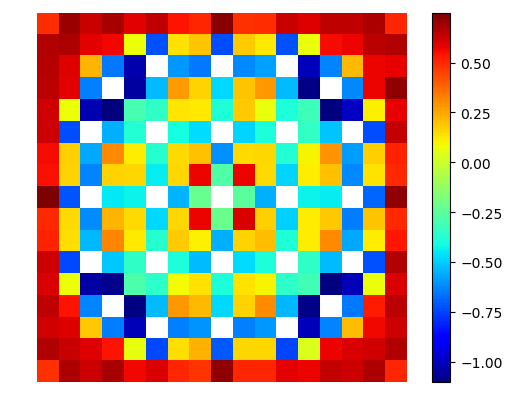
\includegraphics[width=\linewidth]{figures/assembly/capt-null-errors}
  \caption{}
  \label{fig:assm-capt-null-error}
\end{subfigure}
\begin{subfigure}{0.45\textwidth}
  \centering
  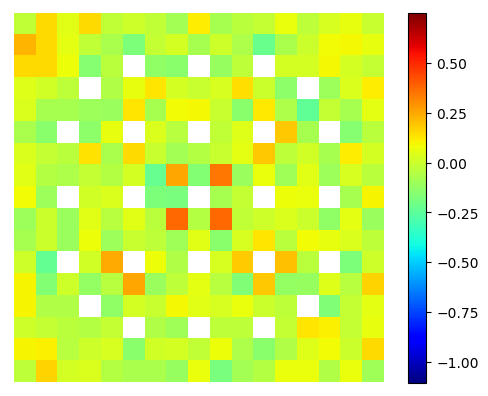
\includegraphics[width=\linewidth]{figures/assembly/capt-degenerate-errors}
  \caption{}
  \label{fig:assm-capt-degen-error}
\end{subfigure}
\begin{subfigure}{0.45\textwidth}
  \centering
  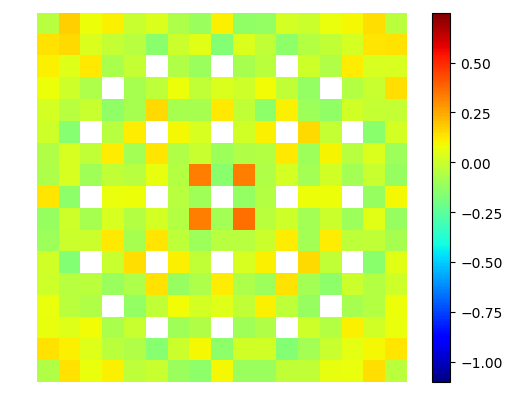
\includegraphics[width=\linewidth]{figures/assembly/capt-lns-errors}
  \caption{}
  \label{fig:assm-capt-lns-error}
\end{subfigure}
\caption{OpenMOC U-238 capture rate percent relative errors for the assembly with null (a), degenerate (b) and LNS (C) spatial homogenization.}
\label{fig:assm-capt-errors}
\end{figure}

\begin{figure}[H]
  \centering 
\begin{subfigure}{0.45\textwidth}
  \centering
  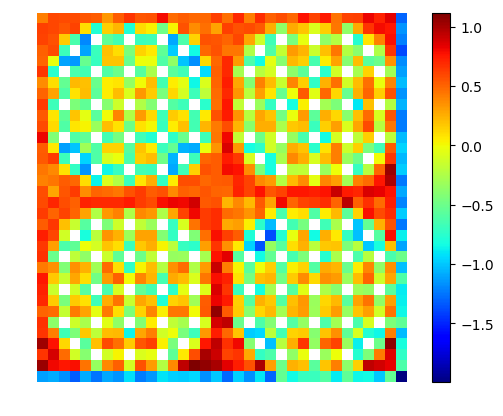
\includegraphics[width=\linewidth]{figures/reflector/capt-null-errors}
  \caption{}
  \label{fig:reflector-capt-null-error}
\end{subfigure}
\begin{subfigure}{0.45\textwidth}
  \centering
  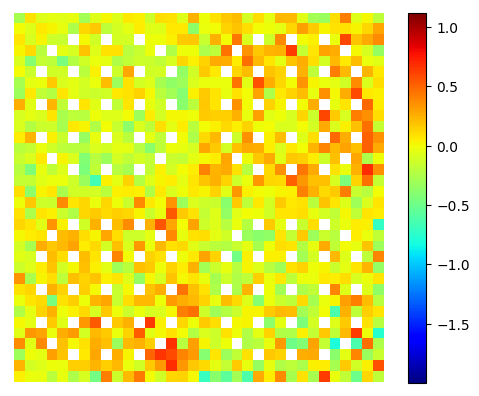
\includegraphics[width=\linewidth]{figures/reflector/capt-degenerate-errors}
  \caption{}
  \label{fig:reflector-capt-degen-error}
\end{subfigure}
\begin{subfigure}{0.45\textwidth}
  \centering
  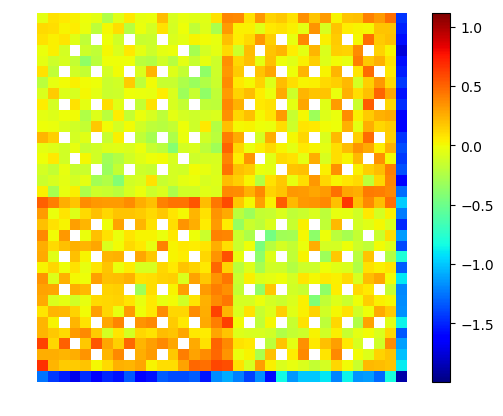
\includegraphics[width=\linewidth]{figures/reflector/capt-lns-errors}
  \caption{}
  \label{fig:reflector-capt-lns-error}
\end{subfigure}
\caption{OpenMOC U-238 capture rate percent relative errors for the colorset with null (a), degenerate (b) and LNS (C) spatial homogenization.}
\label{fig:reflector-capt-errors}
\end{figure}

%%%%%%%%%%%%%%%%%%%%%%%%%%%%%%%%%%%%%%%%%%%%%%%%%%%%%%%%%%%%%%%%%%%%%%%%%%%%%%%
\section{Conclusions}
\label{sec:conclusions}
%%%%%%%%%%%%%%%%%%%%%%%%%%%%%%%%%%%%%%%%%%%%%%%%%%%%%%%%%%%%%%%%%%%%%%%%%%%%%%%

Continuous energy Monte Carlo neutron transport methods have been increasingly applied for multi-group cross section generation. This paper introduced a single-step framework for MC-based MGXS generation for fine-mesh transport codes. The null and degenerate pin-wise spatial homogenization schemes were used to quantify the approximation error due to inter-pin spatial self-shielding effects in PWRs. The Local Neighbor Symmetry (LNS) pin-wise spatial homogenization was introduced to capture many of these self-shielding effects by homogenizing MGXS across groupings of fuel pins with similar neighboring spatial heterogeneities.

%The LNS scheme models spatial self-shielding with fewer materials than degenerate homogenization in order to accelerate the MC tally convergence rate by homogenizing MGXS across many fuel pins.

Two heterogeneous PWR benchmarks -- a fuel assembly and a 2$\times$2 assembly colorset with a water reflector -- were modeled in OpenMOC with MGXS generated by OpenMC. The single-step approach to MGXS generation was employed in which a single Monte Carlo eigenvalue calculation of the entire heterogeneous geometry was employed to collapse cross sections. Null spatial homogenization tallied MGXS for each fuel pin composition, while degenerate homogenization tallied MGXS for each unique fuel pin instance. LNS spatial homogenization applied a geometric template to group fuel pins with similar neighboring spatial heterogeneities. The eigenvalues, fission rates and U-238 capture rates predicted from multi-group calculations with OpenMOC were compared to a reference calculation with OpenMC for each of the three spatial homogenization schemes.

% The pin-wise U-238 capture rates, and to a lesser extent, the pin-wise fission rates, were better predicted when these effects were embedded into MGXS. 

The simulation results presented in this paper demonstrate that global reactivity is preserved when the same MC flux is used to collapse MGXS within a single-step MGXS generation scheme. The OpenMOC eigenvalues for each of the three pin-wise homogenization schemes are consistent to within 10 pcm. Hence, the choice of spatial homogenization technique is inconsequential to eigenvalue predictions. In contrast, the spatial homogenization scheme significantly impacts the accuracy of pin-wise reaction rate predictions. Non-negligible systematic approximation errors in the reaction rates arise when using MGXS which do not account for spatial self-shielding from neighboring fuel pins, control rod guide tubes and reflectors. Degenerate homogenization greatly reduced reaction rate errors with respect to null homogenization since it incorporated perturbations to the flux due to spatial heterogeneities. In particular, the maximum and mean U-238 capture rate errors were reduced by 2 -- 5$\times$ with degenerate homogenization. This demonstrated that the U-238 capture rate errors in deterministic multi-group transport calculations of PWRs are dominated by approximations to spatial self-shielding. In contrast, the fission rates were less sensitive to spatial self-shielding effects, and were only marginally reduced with degenerate homogenization.

LNS spatial homogenization performed as well as degenerate homogenization for a single assembly. However, the scheme failed to distinguish between pins at inter-assembly and assembly-reflector interfaces in the colorset, which resulted in a systematically large U-238 capture rate error for these fuel pins. The difficulty of generalizing the LNS algorithm for arbitrary geometries motivates the need for an unsupervised approach to accurately model spatial self-shielding effects. Such an approach should minimize the number of materials required to account for spatial self-shielding effects, and thus minimize the number of MC particle histories required to sufficiently converge MGXS statistical uncertainties.

%Although degenerate spatial homogenization was shown to be an effective approach to account for inter-pin spatial self-shielding, it is impractical for routine reactor analysis due to computational resource limitations. As a result of the fine-grained spatial tally mesh employed by degenerate homogenization, far more particle histories are needed to converge the MGXS tallies to obtain the same statistical uncertainties as with the simpler null scheme. Nevertheless, this analysis motivates the potential for a new spatial homogenization scheme as accurate as the degenerate scheme but requiring far fewer particle histories to converge MGXS.

%In general, the reaction rate errors for null homogenization are similar for groups of pins with similar neighboring heterogeneities. Hence, the errors may be equivalently reduced if an appropriate set of spatially self-shielded MGXS are defined for groups of pins with similar flux profiles. Future work should develop methods which best identify groups of pins to homogenize to achieve the accuracy of the degenerate scheme while simultaneously approaching the MC convergence rate of the null scheme. This is a topic of ongoing investigation and will be presented in future publications.

%%%%%%%%%%%%%%%%%%%%%%%%%%%%%%%%%%%%%%%%%%%%%%%%%%%%%%%%%%%%%%%%%%%%%%%%%%%%%%%
\section*{Acknowledgments}
%%%%%%%%%%%%%%%%%%%%%%%%%%%%%%%%%%%%%%%%%%%%%%%%%%%%%%%%%%%%%%%%%%%%%%%%%%%%%%%


This work was supported by the Idaho National Laboratory and the National Science Foundation Graduate Research Fellowship Grant No. 1122374. This research made use of the resources of the High Performance Computing Center at Idaho National Laboratory, which is supported by the Office of Nuclear Energy of the U.S. Department of Energy and the Nuclear Science User Facilities under Contract No. DE-AC07-05ID14517.

\section*{References}
\bibliography{references}
\bibliographystyle{annals}

\end{document}
